\documentclass[12pt,a4paper]{report}
\usepackage[top=2.5cm, bottom=2.5cm, right=2cm, left=3.5cm]{geometry}

\usepackage{cmap}
\usepackage[slovak, english, czech]{babel}
\usepackage[utf8]{inputenc}
\usepackage[IL2]{fontenc}
\usepackage{listings}
\usepackage{xcolor}
\usepackage{graphicx}
\usepackage{subcaption}
\usepackage[figurename=Fig.]{caption}
\graphicspath{ {images/} }
\usepackage{float}

\usepackage{color}
\definecolor{lightgray}{rgb}{0.95, 0.95, 0.95}
\definecolor{darkgray}{rgb}{0.4, 0.4, 0.4}
%\definecolor{purple}{rgb}{0.65, 0.12, 0.82}
\definecolor{editorGray}{rgb}{0.95, 0.95, 0.95}
\definecolor{editorOcher}{rgb}{1, 0.5, 0} % #FF7F00 -> rgb(239, 169, 0)
\definecolor{editorGreen}{rgb}{0, 0.5, 0} % #007C00 -> rgb(0, 124, 0)
\definecolor{orange}{rgb}{1,0.45,0.13}      
\definecolor{olive}{rgb}{0.17,0.59,0.20}
\definecolor{brown}{rgb}{0.69,0.31,0.31}
\definecolor{purple}{rgb}{0.38,0.18,0.81}
\definecolor{lightblue}{rgb}{0.1,0.57,0.7}
\definecolor{lightred}{rgb}{1,0.4,0.5}
\usepackage{upquote}

\usepackage{cprotect}

\usepackage{bussproofs}
%\usepackage{lmodern}

\usepackage{Pgfplots}
\usepackage{amsmath}

\usepackage{amsthm}
\newtheorem{veta}{Veta}[section]
\newtheorem{lema}[veta]{Lema}
\theoremstyle{definition}
\newtheorem{definicia}{Definícia}[chapter]
\theoremstyle{remark}
\newtheorem*{poznamka}{Poznámka}

\definecolor{light-gray}{gray}{0.8}

\usepackage{pdfpages}

\usepackage{setspace}
\onehalfspacing
\usepackage{enumitem}

\newcommand*\lif{\mathbin{\to}}
\usepackage{forest}

\forestset{
  smullyan tableaux/.style={
    for tree={
      math content
    },
    where n children=1{
      !1.before computing xy={l=\baselineskip},
      !1.no edge
    }{},
    closed/.style={
      label=below:$\times$
    },
  },
}


\usepackage[hidelinks]{hyperref}

\usepackage{eso-pic}

\newcommand\tab[1][1cm]{\hspace*{#1}}

% CSS
\lstdefinelanguage{CSS}{
  keywords={color,background-image:,margin,padding,font,weight,display,position,top,left,right,bottom,list,style,border,size,white,space,min,width, transition:, transform:, transition-property, transition-duration, transition-timing-function}, 
  sensitive=true,
  morecomment=[l]{//},
  morecomment=[s]{/*}{*/},
  morestring=[b]',
  morestring=[b]",
  alsoletter={:},
  alsodigit={-}
}

% JavaScript
\lstdefinelanguage{JavaScript}{
  morekeywords={typeof, new, true, false, catch, function, return, null, catch, switch, var, if, in, while, else, case, break},
  morecomment=[s]{/*}{*/},
  morecomment=[l]//,
  morestring=[b]",
  morestring=[b]'
}

\lstdefinelanguage{HTML5}{
  language=html,
  sensitive=true,   
  alsoletter={<>=-},    
  morecomment=[s]{<!-}{-->},
  tag=[s],
  otherkeywords={
  % General
  <, >,
  % Standard tags
    <!DOCTYPE,
  </html, <html, <head, <title, </title, <style, </style, <link, </head, <meta, />,
    % body
    </body, <body,
    % Divs
    </div, <div, </div>, 
    % Paragraphs
    </p, <p, </p>,
    % scripts
    </script, <script,
  % More tags...
  <b, </b, <strong, </strong, <small, </small, <i, </i, <canvas, /canvas>, <svg, <rect, <animateTransform, </rect>, </svg>, <video, <source, <iframe, </iframe>, </video>, <image, </image>, <header, </header, <article, </article, 
  <w, </w, <s, </s
  },
  ndkeywords={
  % General
  =,
  % HTML attributes
  charset=, src=, id=, width=, height=, style=, type=, rel=, href=,
  % SVG attributes
  fill=, attributeName=, begin=, dur=, from=, to=, poster=, controls=, x=, y=, repeatCount=, xlink:href=,
  % properties
  margin:, padding:, background-image:, border:, top:, left:, position:, width:, height:, margin-top:, margin-bottom:, font-size:, line-height:,
    % CSS3 properties
  transform:, -moz-transform:, -webkit-transform:,
  animation:, -webkit-animation:,
  transition:,  transition-duration:, transition-property:, transition-timing-function:,
  }
}

\lstdefinestyle{htmlcssjs} {%
  % General design
%  backgroundcolor=\color{editorGray},
  basicstyle={\fontsize{10}{11}\ttfamily},   
  frame=b,
  % line-numbers
  xleftmargin={0.75cm},
  numbers=left,
  stepnumber=1,
  firstnumber=1,
  numberfirstline=true, 
  % Code design
  identifierstyle=\color{black},
  keywordstyle=\color{blue}\bfseries,
  ndkeywordstyle=\color{editorGreen}\bfseries,
  stringstyle=\color{editorOcher}\ttfamily,
  commentstyle=\color{brown}\ttfamily,
  % Code
  language=HTML5,
  alsolanguage=JavaScript,
  alsodigit={.:;},  
  tabsize=2,
  showtabs=false,
  showspaces=false,
  showstringspaces=false,
  extendedchars=true,
  breaklines=true,
  % German umlauts
  literate=%
  {á}{{\'a}}1 {é}{{\'e}}1 {í}{{\'i}}1 {ó}{{\'o}}1 {ú}{{\'u}}1
  {Á}{{\'A}}1 {É}{{\'E}}1 {Í}{{\'I}}1 {Ó}{{\'O}}1 {Ú}{{\'U}}1
  {à}{{\`a}}1 {è}{{\`e}}1 {ì}{{\`i}}1 {ò}{{\`o}}1 {ù}{{\`u}}1
  {À}{{\`A}}1 {È}{{\'E}}1 {Ì}{{\`I}}1 {Ò}{{\`O}}1 {Ù}{{\`U}}1
  {ä}{{\"a}}1 {ë}{{\"e}}1 {ï}{{\"i}}1 {ö}{{\"o}}1 {ü}{{\"u}}1
  {Ä}{{\"A}}1 {Ë}{{\"E}}1 {Ï}{{\"I}}1 {Ö}{{\"O}}1 {Ü}{{\"U}}1
  {â}{{\^a}}1 {ê}{{\^e}}1 {î}{{\^i}}1 {ô}{{\^o}}1 {û}{{\^u}}1
  {Â}{{\^A}}1 {Ê}{{\^E}}1 {Î}{{\^I}}1 {Ô}{{\^O}}1 {Û}{{\^U}}1
  {œ}{{\oe}}1 {Œ}{{\OE}}1 {æ}{{\ae}}1 {Æ}{{\AE}}1 {ß}{{\ss}}1
  {ű}{{\H{u}}}1 {Ű}{{\H{U}}}1 {ő}{{\H{o}}}1 {Ő}{{\H{O}}}1
  {ç}{{\c c}}1 {Ç}{{\c C}}1 {ø}{{\o}}1 {å}{{\r a}}1 {Å}{{\r A}}1
  {€}{{\euro}}1 {£}{{\pounds}}1 {«}{{\guillemotleft}}1
  {»}{{\guillemotright}}1 {ñ}{{\~n}}1 {Ñ}{{\~N}}1 {¿}{{?`}}1
  {á}{{\'a}}1
         {ľ}{{\v{l}}}1
         {Ľ}{{\v{L}}}1
         {í}{{\'i}}1
         {ĺ}{{\'l}}1
         {Ĺ}{{\'L}}1
         {ŕ}{{\'r}}1
         {Ŕ}{{\'R}}1
         {é}{{\'e}}1
         {ý}{{\'y}}1
         {ú}{{\'u}}1
         {ó}{{\'o}}1
         {ě}{{\v{e}}}1
         {š}{{\v{s}}}1
         {č}{{\v{c}}}1
         {ř}{{\v{r}}}1
         {ž}{{\v{z}}}1
         {ď}{{\v{d}}}1
         {ť}{{\v{t}}}1
         {ň}{{\v{n}}}1                
         {ů}{{\r{u}}}1
         {Á}{{\'A}}1
         {Í}{{\'I}}1
         {É}{{\'E}}1
         {Ý}{{\'Y}}1
         {Ú}{{\'U}}1
         {Ó}{{\'O}}1
         {Ě}{{\v{E}}}1
         {Š}{{\v{S}}}1
         {Č}{{\v{C}}}1
         {Ř}{{\v{R}}}1
         {Ž}{{\v{Z}}}1
         {Ď}{{\v{D}}}1
         {Ť}{{\v{T}}}1
         {Ň}{{\v{N}}}1                
         {Ů}{{\r{U}}}1  
}

\makeatletter
\g@addto@macro\@floatboxreset{\centering}
\makeatother
\begin{document}

%\includepdf{zadanie.pdf}

%%% DEFINÍCIE NÁZVOV
\def\nazov{Jednoduchý syntaktický parser príbehov z Multimediálnej čítanky}
\def\autor{Martin Heinz}
\def\skolitel{RNDr.~Marek Nagy,~PhD.}
\def\katedra{Katedra Aplikovanej Informatiky}
\def\fakulta{Fakulta matematiky, fyziky a~informatiky}
\def\univerzita{Univerzita Komenského v~Bratislave}
\def\mesto{Bratislava}
\def\typprace{Bakalárska práca}
\def\rok{2016}
%%% OBAL
\thispagestyle{empty}
\begin{center}
\textsc{\LARGE\univerzita}\\
\bigskip\textsc{\LARGE\fakulta}\\
\vfill\textsc{\Huge\nazov}\\
\medskip{\Large\typprace}\\
\vfill{\large\rok\hfill\autor}
\end{center}
%%% TITULNÝ LIST
\newpage
\thispagestyle{empty}
\begin{center}
\textsc{\LARGE\univerzita}\\
\medskip\textsc{\LARGE\fakulta}\\
\vskip 0cm plus 2fill\textsc{\Huge\nazov}\\
\medskip{\Large\typprace}\\

\vskip 0cm plus 1fill
\begin{tabular}{ll}
%Evidenčné číslo: & ... \\
Študijný program: & Aplikovaná informatika\\
Študijný odbor: & 9.2.9. aplikovaná informatika\\
Školiace pracovisko: & \katedra\\
Školiteľ: & \skolitel
\end{tabular}\\
\vskip 0cm plus 1fill{\large\mesto{} \rok\hfill\autor}
\end{center}

%\begin{figure}[hbtp]
%\centering
%\vspace{-2cm}
%\hspace{-2cm}
\includegraphics[width=1.1\textwidth]{pracaScanAdjusted}
%\end{figure}


%\AddToShipoutPictureBG{%
%  \AtPageLowerLeft{
\includegraphics[width=\paperwidth,height=\paperheight]{pracaScanAdjusted}}
%  }
\newpage 
\thispagestyle{empty}

\begin{figure}[hbtp]

\includepdf[offset=0 -75]{pracaScanAdjusted}
\end{figure}


\chapter*{Poďakovanie}
\thispagestyle{empty}
Chcel by som sa poďakovať môjmu školiteľovi, RNDr. Marekovi Nagyovi, PhD., za svoj čas, trpezlivosť, cenné rady, pripomienky a usmernenia pri tvorbe tejto bakalárskej práce.

\newpage
{~}\vfill
{\noindent \large\bf Čestné vyhlásenie} 
\vspace{1.5cm}

Čestne prehlasujem, že som túto bakalársku prácu vypracoval samostatne s použitím uvedených zdrojov.\\\\ 
V Bratislave
\hfill ................................... 
\vspace{1cm}

\begin{abstract}

Cieľom tejto bakalárskej práce je vytvoriť syntaktický parser v jazyku JavaScript, ktorý bude využitý ako modul na parsovanie príbehov v aplikácii Multimediálna čítanka.
Táto práca obsahuje popis a analýzu problematiky a  parsovacieho algoritmu použitého pri tvorbe tejto aplikácie. Súčasťou práce je aj návrh a implementácia samotnej aplikácie.


Táto aplikácia je navrhnutá s cieľom implementovať efektívnu metódu delenia komplexného textu obsahujúceho HTML značky na slová a vety s jednoduchým používaním a modifikovateľnosťou.

\bigskip\noindent
\textbf{Kľúčové slová:} \textit{parser, javascriptová aplikácia, HTML, XML} 

\bigskip
HEINZ, Martin: \nazov \  [Bakalárska práca]. Fakulta
matematiky, fyziky a informatiky Univerzita Komenského v Bratislave; Katedra aplikovanej
informatiky. Školiteľ: \skolitel \ Bratislava 2017. TODO DOPLNIT strán.

\end{abstract}

\begin{otherlanguage}{english}
\begin{abstract}

Goal of this work is to create a syntactic parser in JavaScript, which is intened to be used as a submodule for parsing of stories in Multimedia reader. This work contains description and analysis of issues and parsing algorithm used for development of this application. This work also contains design and implentation of application itself.


This application is developed with goal of implementing effective method to split complex text containing HTML tags into words and sentences, while being easy to use and modify.

\bigskip\noindent
\textbf{Keywords:} \textit{parser, javascript, HTML, XML} 

\bigskip
HEINZ, Martin: Simple Syntactic Parser of Stories from Multimedia Reader [Bachelor thesis]. Faculty of Mathematics, Physics and Informatics;
Department of Applied Informatics, Comenius University in Bratislava; Supervisor: \skolitel \ Bratislava 2017. TODO DOPLNIT pages.

\end{abstract}
\end{otherlanguage}
\setcounter{tocdepth}{1}
\tableofcontents

\chapter*{Úvod}
\addcontentsline{toc}{chapter}{\protect\numberline{}Úvod}
V dnešnej dobe je spracovávanie textu bežnou vecou, s ktorou sa stretávame veľmi často a vo veľa rôznych situáciách. Mnohé aplikácie pre svoje správne fungovanie potrebujú text rozdelený do nejakých menších celkov, napríklad viet a slov. Vo veľa prípadoch však správnosť, prípadne efektívnosť takéhoto spracovania nie je na dostatočnej úrovni a ani zďaleka sa nepribližuje presnosti, s ktorou vie takýto text spracovať človek, ktorý však ďaleko zaostáva za počítačmi v efektívnosti.
\bigskip


Hlavným cieľom tejto bakalárskej práce je vytvoriť aplikáciu  - syntaktický parser - ktorá bude využitá na parsovanie príbehov z Multimediálnej čítanky, ktoré bude schopná s čo najväčšou presnosťou a efektívnosťou deliť na jednotlivé slová a vety, so zachovaním pôvodného formátovania textu a s dôrazom na univerzálnosť tohoto riešenia.
\bigskip


Práca je rozdelená do štyroch kapitol. Prvá z nich sa zaoberá cieľom, problematikou parsovania, porovnaním jednotlivých parsovacích algoritmov a analýzou algoritmu zvoleného pre túto aplikáciu. Táto kapitola tiež zahŕňa prehľad existujúcich podobných systémov a stručný náhľad na použité technológie potrebné pri implementácii výslednej aplikácie. Druhá kapitola je zameraná na návrh a samotnú implementáciu. V tejto kapitole sú predstavené jednotlivé časti aplikácie, ich funkcionalita a popis realizácie niektorých funkcií. Posledná kapitola pozostáva z testov a porovnaní  efektívnosti samotného riešenia.
\bigskip


Záver tejto bakalárskej práce poskytuje zhodnotenie naplnenia stanovených cieľov, ako aj pohľad na ďalšie možnosti vývoja v tejto oblasti.
%\setcounter{page}{5}

\chapter{Východiská}
\section{Cieľ}


Cieľom tejto práce je nájdenie vhodného parseru, ktorý by bol v čo najkratšom čase schopný rozdeľovania komplexného textu na vety a slová a vytvorenie aplikácie pozostávajúcej z tohoto parseru, jeho gramatiky(slovenskej aj anglickej) a slovníku a časti spracovávajúcej výstup parseru do výsledného XML dokumentu. Zároveň by gramatika aj slovník parseru mali byť ľahko modifikovateľné a mala by existovať aj možnosť pridávať ďalšie jazyky. Príklad vstupu a výstupu:
\begin{lstlisting}[caption={Vstup},style=htmlcssjs, label={lst:vstup}]
Toto <p> je vstupný text. Obsahuje čísla, napr.: č. 1, 5.(piaty), alebo mená - M. Heinz a aj priamu reč... </p>
Eva sa <b> pýtala: - Čo ti povedali!?</b>
"Ahoj," povedal, "ako sa..." skočil mu do reči, "<i>ticho!</i>"
- Prídeš? - spýtal sa.
- Prídem.
\end{lstlisting}
\begin{lstlisting}[caption={Výstup},style=htmlcssjs, label={lst:vystup}]
<p><s id="s1"><w id="w1">Toto</w><w id="w2">je</w><w id="w3">vstupný</w><w id="w4">text</w>.</s>
["Obsahuje", "čísla", "napr.", ":", "č.", "1", ",",  "5.", "(", "piaty", ")", ",", "alebo", "mená", "-", "M.", "Heinz", "a", "aj", "priamu", "reč", "..."]</p>
[["Eva", "sa","<b>", "pýtala", ":", "</b>"], ["<b>", "-", "Čo", "ti", "povedali", "?!", "</b>"]]
[["Ahoj", ",", "\""],
	["povedal", ","],
	["\"","ako", "sa", "...", "\""],
	["skočil", "mu", "do", "reči", ","],
	["\"", "<i>", "ticho", "!", "</i>", "\""]]
[["-", "Prídeš", "?"],
	["-", "spýtal", "sa", "."]]
["-", "Prídem", "."]
\end{lstlisting}
\noindent \textit{Poznámka: Všetko okrem prvej vety je uvedené vo forme polí kvôli čitateľnosti. Skutočný výstup by mal rovnakú štruktúru ako prvá uvedená veta.}

\section{Prehľad problematiky}
\subsection{Syntaktický parser}
V tejto časti sa budem snažiť popísať, čo vlastne parsovanie je a na akom princípe pracuje, zároveň vysvetlím aj dôležité pojmy, ktoré budem v práci používať. Rozoberiem niektoré spôsoby parsovania, ich výhody a nevýhody. Tiež podrobnejšie vysvetlím vybraný algoritmus použitý na vytvorenie aplikácie.

\subsection{Čo je to parsovanie?}
Parsovanie ako pojem popisuje proces tvorby syntaktickej analýzy vety na základe vopred danej formálnej gramatiky(Context-free Grammar - CFG) a slovníku. Výsledná  syntaktická analýza môže byť použitá pre ďalšiu sémantickú interpretáciu. V tejto práci sa však budeme zaoberať len syntaktickou analýzou pomocou CFG, keďže našim cieľom nie hlbšia analýza slov. \cite{Pulman}\cite{Girju}

\subsection{Context-free grammar}
Context-free grammar\cite{foja}, skrátene CFG je typ formálnej gramatiky. Je to množina substitučných pravidiel, ktoré popisujú všetky existujúce reťazce v danom jazyku. Príklady substitučných pravidiel:
$$ A \to \alpha $$
$$ A \to \beta $$

Toto označuje, že môžeme vymeniť $A$ za $\alpha$ alebo $\beta$ \\ \\
V CFG sú všetky pravidlá jedna k jednej, jedna k veľa alebo jedna k ničomu(epsilon rule). Ľavá strana pravidla je vždy neterminálny symbol. Našimi terminálnymi symbolmi budú napríklad slová, čísla alebo interpunkčné znamienka. Príklad CFG:

$$ G = (N, \Sigma , R, S) $$

kde:
\begin{itemize}
\item $N$ je množina neterminálnych symbolov
\item $\Sigma$ je množina terminálnych symbolov
\item $R$ je množina pravidiel v tvare $X \to Y_1 Y_2 \dots Y_n$ pre $ n \geq 0 \in N, Y_i \in ( N \cup \Sigma )$
\item $S$ je začiatočný symbol, ktorý reprezentuje celý vstupný reťazec. $S$ musí patriť do $N$
\end{itemize}

\noindent Konkrétnejší príklad - zadefinujme si nasledujúce substitúcie:

$$ S \to AB $$
$$ A \to a $$
$$ A \to aA $$
$$ B \to b $$
$$ B \to bB $$

V tomto prípade $A$ a $B$ sú premenné a $S$ je začiatočná premenná. $a$ a $b$ sú terminály. Využijeme vyššie uvedené pravidlá na nájdenie reťazcov skladajúcich sa z terminálov nasledujúcim spôsobom:
\begin{itemize}
\item Začneme použitím začiatočnej premennej $S$(inicializácia reťazca).
\item Zoberieme ktorúkoľvek premennú v aktuálnom reťazci a vyberieme hociktoré pravidlo, ktoré má túto premennú na ľavej strane, následne nahradíme túto premennú pravou stranou tohoto pravidla.
\item Opakujeme predchádzajúci krok, až kým sa v reťazci nenachádzajú len terminály.
\end{itemize}

Napríklad reťazec $aaaabb$ môže vzniknúť z vyššie uvedených pravidiel takto:

$$ S \to AB $$
$$ AB \to aAB $$
$$ aAB \to aAbB $$
$$ aAbB \to aaAbB $$
$$ aaAbB \to aaaAbB $$
$$ aaaAbB \to aaaabB $$
$$ aaaabB \to aaaabb $$
\subsection{Parse Tree}
Parse tree alebo strom odvodenia je strom reprezentujúci syntaktickú štruktúru reťazca podľa nejakej formálnej gramatiky. V parsovacom strome koreň reprezentuje začiatočný symbol, všetky vnútorné vrcholy sú označené neterminálnými symbolmi gramatiky, potomkovia týchto vrcholov sú časťami pravej strany použitého substitučného pravidla usporiadané zľava doprava. Listami stromu sú samotné terminály. Príklad stromu na obrázku (\ref{fig:strom})
\subsection{Typy parserov}
\subsubsection*{Top-down parser} 
\addcontentsline{toc}{subsubsection}{Top-down parser}
Názov tohto parseru vychádza zo spôsobu akým vytvára parsovací strom, teda zhora nadol.
Princíp top-down parseru je možné popísať takto: Začíname so štartovacím symbolom $S$, pozrieme sa aký symbol sa nachádza na pravej strane úvodného pravidla (1.1), ďalej si zoberieme prvé pravidlo začínajúce týmto symbolom($Sum$ (1.2)) a pozrieme sa či sa prvý symbol jeho substitúcie zhoduje s tokenom v našom vstupe, ak áno, tak pokračujeme ďalším symbolom substitúcie ak nie, tak musíme vyskúšať ďalšie pravidlá(1.3)
\begin{align}
S \to Sum \\
Sum \to Sum [+-] Product \\
Sum \to Product \\
Product \to Product [*/] Factor \\
Product \to Factor \\
Factor \to "(" Sum ")" \\
Factor \to Number \\
Number \to [0-9]+
\end{align}
\noindent 
Príklad pre vstup: $ 5 + (3 * 2)$ a príklad stromu, ktorý vznikne pre tento vstup: \\

\begin{figure}[H]
\centering
\begin{minipage}{0.47\textwidth}
  \centering
  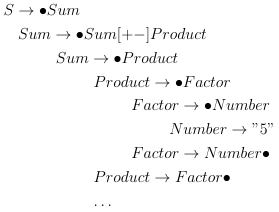
\includegraphics[width=\textwidth]{mathTree}
  \captionof{figure}{Príklad pre vstup $ 5 + (3 * 2)$}
  \label{fig:test1}
\end{minipage}%
\hfill
\begin{minipage}{0.35\textwidth}
  \centering
  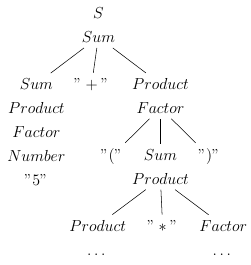
\includegraphics[width=\textwidth]{mathForest}
  \captionof{figure}{Príklad stromu}
  \label{fig:strom}
\end{minipage}
\end{figure}

%\noindent 
%
%$ S \to \bullet Sum $ \\
%\tab $ Sum \to \bullet Sum [+-] Product $ \\
%\tab \tab $Sum \to \bullet Product$ \\
%\tab \tab \tab $Product \to \bullet Factor$ \\
%\tab \tab \tab \tab $Factor \to \bullet Number$ \\
%\tab \tab \tab \tab \tab $Number \to "5"$ \\
%\tab \tab \tab \tab $Factor \to  Number \bullet$ \\
%\tab \tab \tab $Product \to Factor \bullet$ \\
%\tab \tab \tab \dots \\

% Toto je parsovací strom, ktorý by vznikol pre tento vstup: 
%\begin{center}
%\begin{forest}
%  smullyan tableaux
%[S
%	[ Sum
%		[ Sum
%			[Product
%				[ Factor
%					[Number
%						["5"]
%					]
%				]
%			]
%		]
%		["+"
%		]
%		[Product
%			[Factor
%				["("
%				]
%				[Sum
%					[Product
%						[Product
%							[\dots]
%						]
%						["*"
%						]
%						[Factor
%							[\dots]
%						]
%					]
%				]
%				[")"
%				]
%			]
%		]
%	]
%]
%\end{forest}
%\end{center}

V tomto príklade sme ale v každom kroku vybrali správne pravidlo, ktoré by nás doviedlo k výsledku, v skutočnosti by sme pri naivnom algoritme museli vyskúšať všetky možnosti.


\textit{Poznámka: Vo všetkých príkladoch budem pre ľahkú pochopiteľnosť využívať jednoduchú aritmetiku pre CFG(popísané nižšie).} 
\subsubsection*{Bottom-up parser} 
\addcontentsline{toc}{subsubsection}{Bottom-up parser}

Bottom-up parser zjavne, už podľa názvu skladá parsovací strom odspodu nahor, presnejšie od ľavého dolného rohu. Základný princíp je takýto: zoberieme si token zo vstupu a pokúsime sa nájsť zhodu na pravej strane pravidiel, ak sa nám podarí nahradiť celú pravú stranu, vymeníme túto sekvenciu symbolov za ľavú stranu použitého pravidla, toto opakujeme až kým nevytvoríme celý strom. V konečnom dôsledku získame rovnaký parsovací strom ako pri top-down parsery.

\subsection{Chart parser} 
\addcontentsline{toc}{subsubsection}{Chart parser}
Chart parser je typ parseru vhodný pre nejednoznačné gramatiky(natural language processing). Kvôli efektívnosti využíva dynamické programovanie pre zapamätanie čiastočných hypotetických parsov. Tieto čiastočné riešenia si pamätá v tabuľke - z toho názov Chart parser. Bližší popis konkrétneho Chart parseru v ďalšej sekcii(\ref{sec:earley}).

\subsection{Earley parser}
\label{sec:earley}

Earley parser\cite{Vaillant} patrí medzi top-down chart parsery. Je schopný parsovať akýkoľvek Context-free grammar, teda je veľmi vhodný pre parsovanie prirodzeného jazyka. V porovnaní s obyčajnými top-down alebo bottom-up parsermi je aj vcelku efektívny - jeho výpočtová zložitosť je $O(n^3)$, kde $n$ je dĺžka parsovaného reťazca, s tým, že pre jednoznačné gramatiky to je $O(n^2)$.

\subsubsection*{Earley items} 
Tak ako už bolo povedané, chart parsery si pamätajú zoznam čiastočných parsov. To isté robí aj Earley parser, prvky týchto zoznamov sa nazývajú Earley items.

$$ Sum \to Sum \bullet [+-] Product \tab  (0)  $$

\begin{itemize}
\item Číslo v zátvorkách označuje, kde tento Earley item začal - v tomto prípade je to $(0)$, teda úplný začiatok vstupného reťazca.
\item tučná bodka označuje koľko už bolo zo vstupu vyparsované, teda všetko naľavo od bodky už je hotové. 
\end{itemize}

\subsubsection*{State sets}

State sety sú množiny Earley item-ov. Sú uložené v dynamickom poli, ktoré môžeme nazvať jednoducho $S$. Toto je možná reprezentácia:

\begin{figure}[h]
\centering
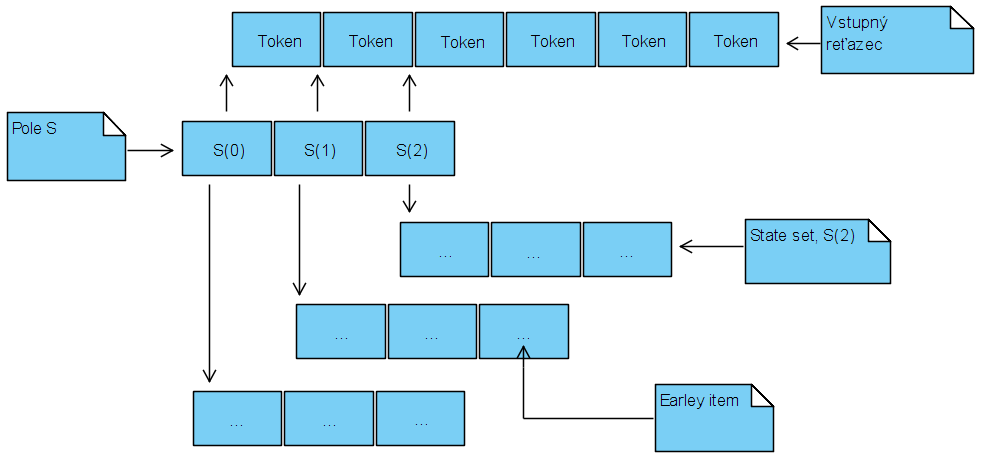
\includegraphics[scale=0.75]{stateSet}
\caption{Príklad reprezentácie}
\end{figure}

\subsubsection*{Pridávanie Earley item-ov}
Existujú 3 spôsoby ako môžeme pridať nové Earley item-y do state setov, ktorý spôsob použijeme záleží na tom čo očakávame v našich pravidlách(čo sa nachádza napravo od tučnej bodky).

\subsubsection*{Prediction}
Prvou z troch možností je predikcia - symbol napravo od bodky je neterminál. Pridáme pravidlo prislúchajúce k tomuto neterminálu do aktuálneho state setu.

\begin{figure}[h]
\centering
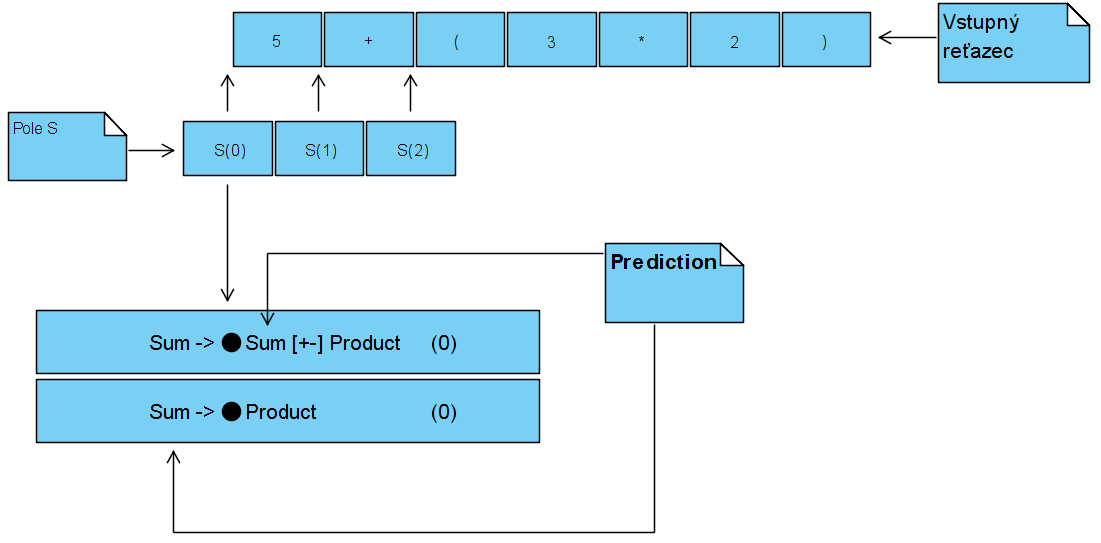
\includegraphics[scale=0.7]{prediction}
\caption{Príklad predikcie}
\end{figure}
\subsubsection*{Scan}
Druhá možnosť - symbol napravo od bodky je terminál. Skontrolujeme či sa token na vstupe zhoduje s daným terminálom, ak áno pridáme tento Earleyho item, posunutý o jeden krok do ďalšieho state setu.

\begin{figure}[h]
\centering
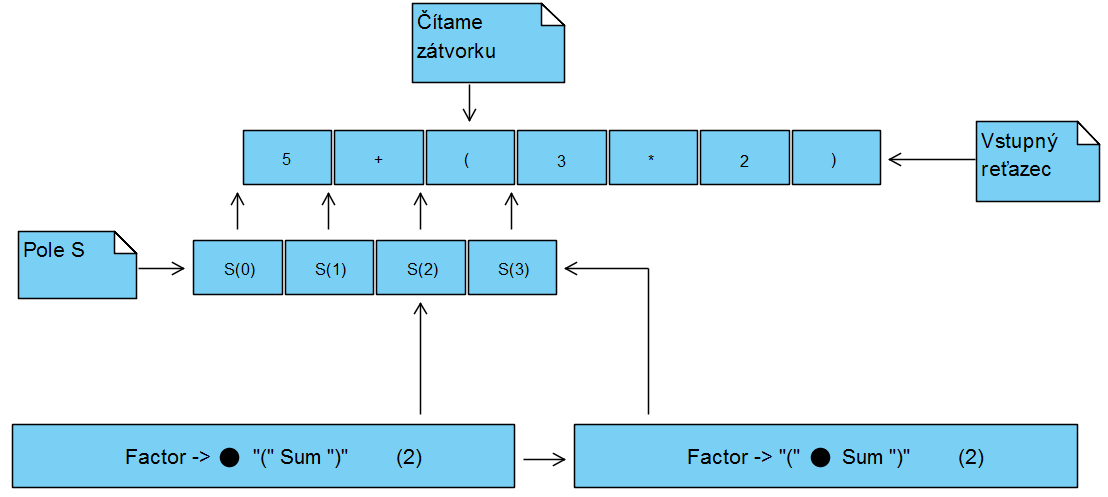
\includegraphics[scale=0.7]{scan}
\caption{Príklad scanu}
\end{figure}

\subsubsection*{Completion}
Posledná možnosť - napravo od bodky už nie je nič. To znamená, že sme dokončili čiastočný pars. Pokúsime sa nájsť rodiča tohto item-u a pridáme ho do aktuálneho state setu, s tým že ho posunieme o krok dopredu.

\begin{figure}[H]
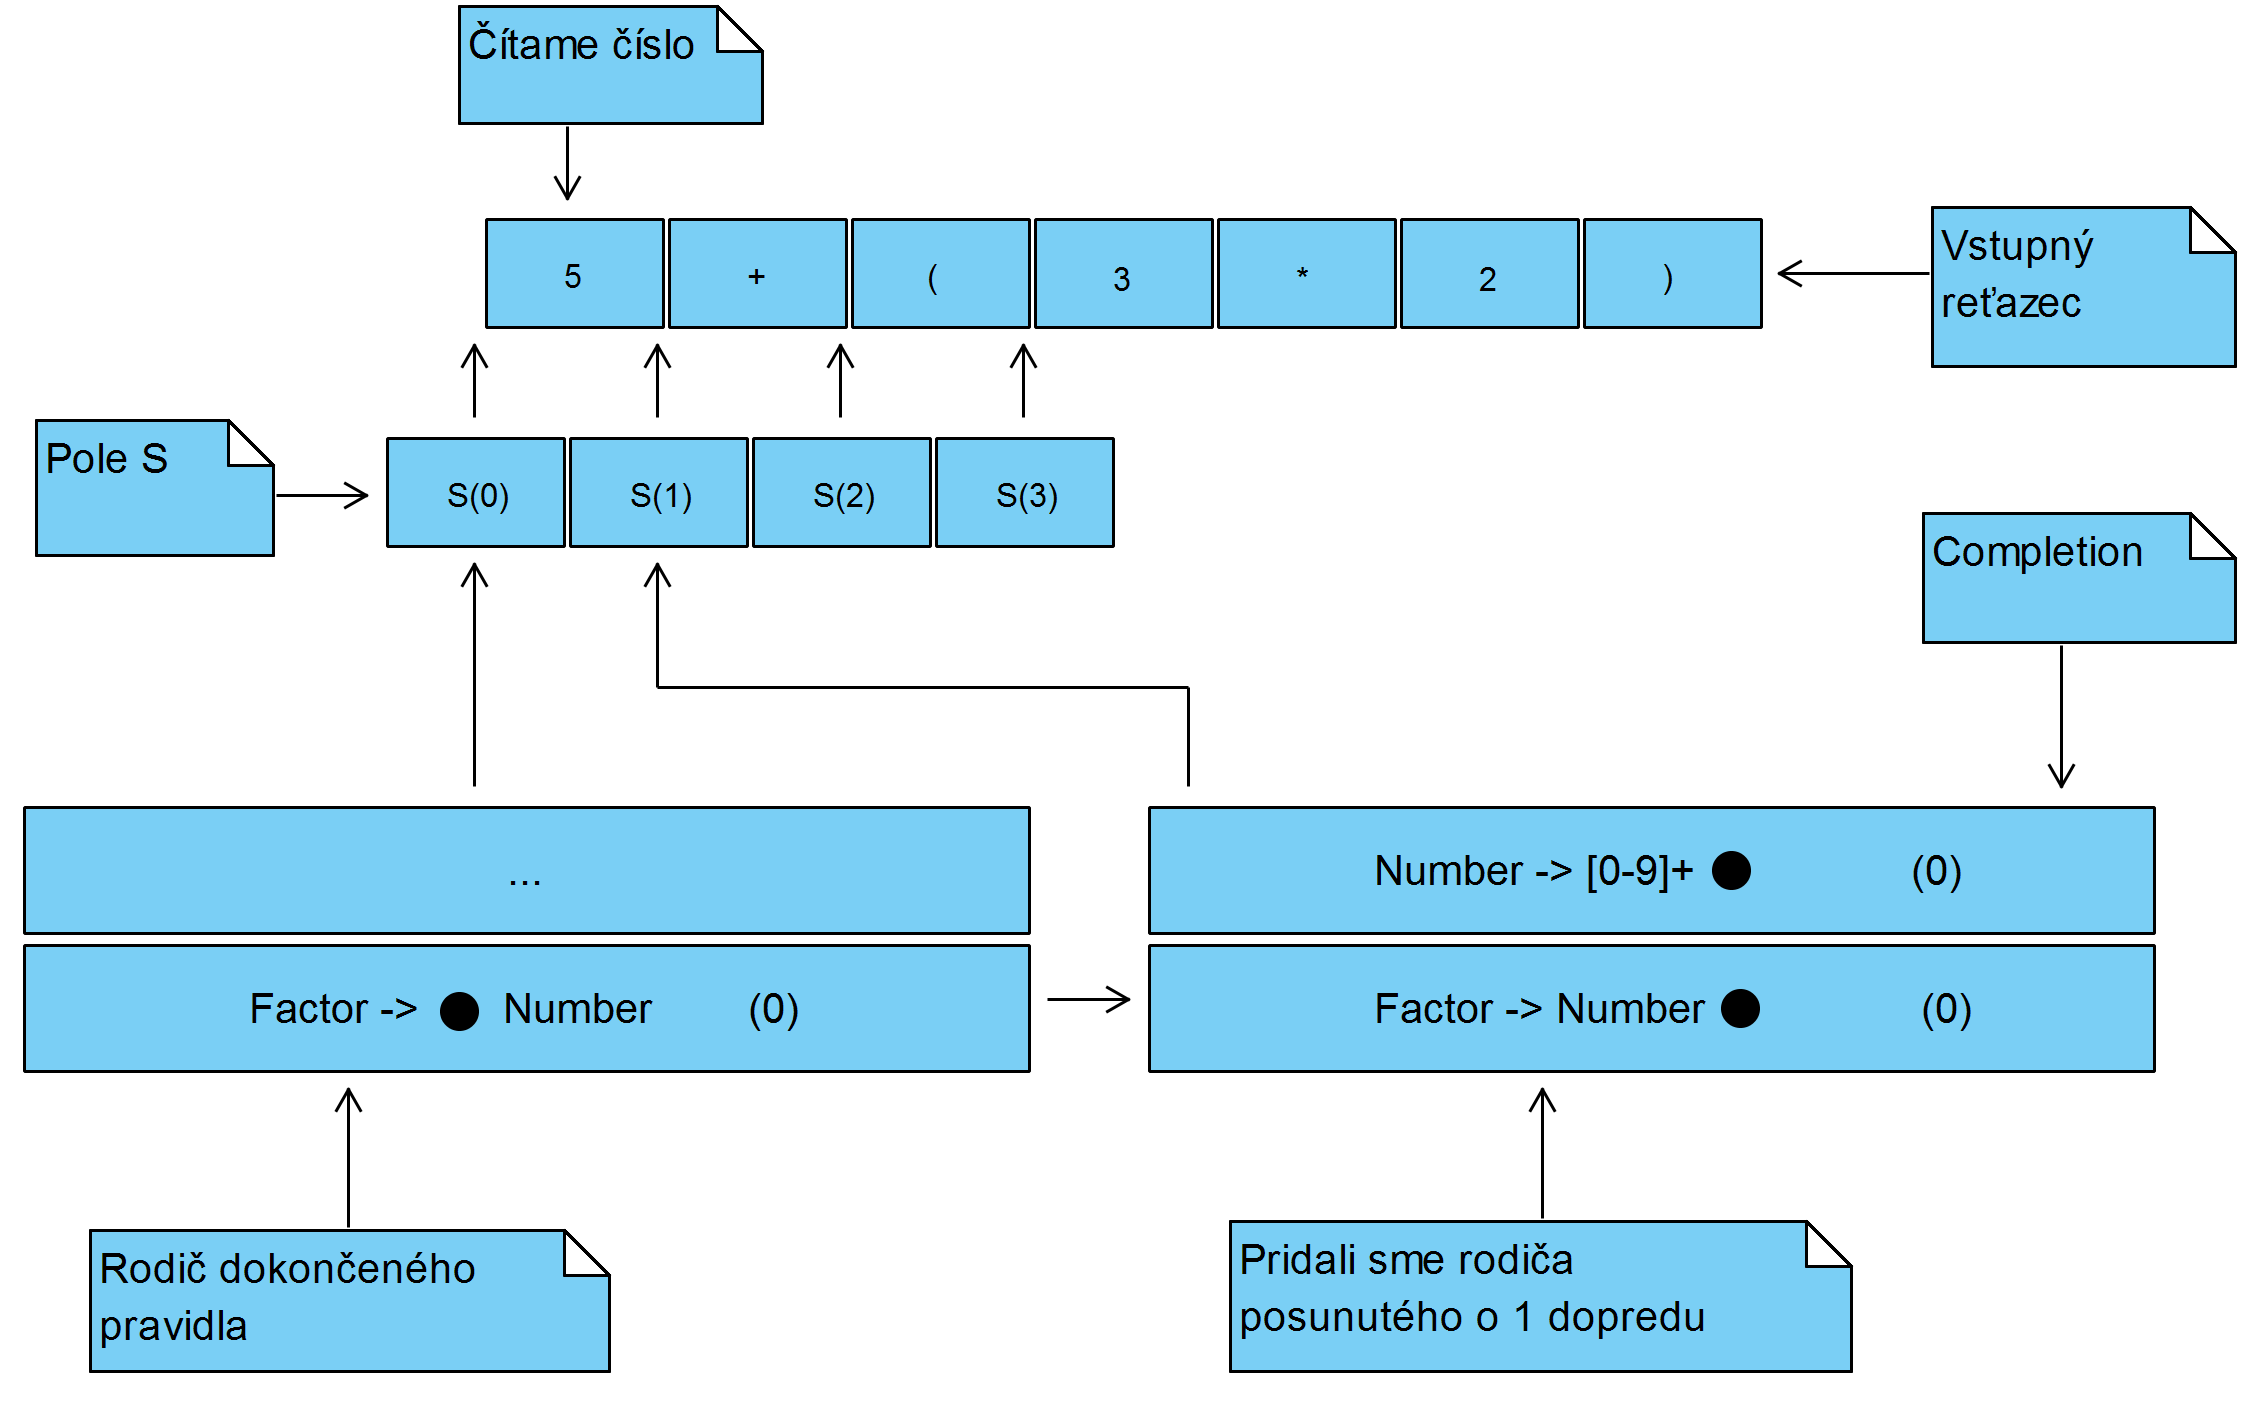
\includegraphics[scale=0.7]{completition}
\caption{Príklad completion}
\end{figure}

\subsubsection*{Failure modes} 
Existujú dve situácie kedy môže parser zlyhať:
\begin{itemize}
\item Nepodarí sa vyparsovať celý vstup. To sa môže stať ak je vo vstupe chyba(vstup nedáva zmysel), napríklad: $"5 + ()"$
\item Podarí sa vyparsovať celý vstup, ale nevznikne kompletný pars, napríklad: $"5 *"$ - toto je korektný začiatok vstupu($Product$ z našej ukážkovej gramatiky), ale na dokončenie nám chýba posledný token.
\end{itemize}

\subsection{Porovnanie parserov}
Za zmienku stoja aj ďalšie parsovacie algoritmy, ktoré však majú určité nevýhody, čím robia z Earley parseru najlepšiu voľbu pre túto aplikáciu:
\begin{itemize}
\item CYK algorithm: Má síce tiež výpočtovú zložitosť ako Earley, ale pamäťová zložitosť je $O(n^2)$, pričom u Earley parseru to je len $O(n)$ \cite{complexity}. CYK zároveň potrebuje gramatiku v CNF, kde Earley funguje pre akúkoľvej gramatiku a tak ako už bolo spomenuté skôr, tak pre niektoré gramatiky parsuje aj s lepšou zložitosťou ako $O(n^3)$.
\item LR parser: Je síce schopný parsovať vstupný reťazec v lineárnom čase, ale nie je dostatočne flexibilný pre parsovanie prirodzeného jazyka(je vhodnejší pre programovacie jazyky)
\item LL parser: Je veľmi jednoduchý, nie je však schopný parsovať akýkoľvek context-free grammar.
\item Valiant’s algorithm: (Teoreticky)Rýchlejší algoritmus než Earley algorithm použiteľný pre natural language processing. Algoritmus má výpočtovú zložitosť $O(n^{2.81})$, čo je lepšie ako Earley algorithm, ale jeho koeficienty sú také veľké, že v praxi by bol rýchlejší len pre obrovské vstupy.\cite{Tomita}
\end{itemize}

\section{Prehľad existujúcich systémov}
V nasledujúcej podkapitole sa budem venovať existujúcim riešeniam podobného problému. Medzi takéto riešenia môžeme zaradiť rôzne syntaktické parsery alebo knižnice určené pre natural language processing.

\subsection{Nearly.js}
Nearly.js je parsovací tool kit využívajúci Earley parser napísaný v JavaScripte. Parser využíva vlastnú gramatiku a umožňuje používanie makier. Je tiež schopný parsovať nejednoznačnú gramatiku a vracia v tomto prípade všetky parsy. Nearly tiež umožňuje debugovanie a má aj určitú detekciu chýb. Ďalšou funkcionalitou je aj možnosť konvertovať gramatiku na čitateľnejšie SVG "koľajnicové" diagramy.

\subsection{Stanford CoreNLP}
Stanford CoreNLP poskytuje viaceré nástroje pre natural language processing. Je napísaný v Jave, s tým, že poskytuje interface aj ďalšie programovacie jazyky. Medzi funkcionality CoreNLP patrí aj part-of-speech tagger, named entity recognizer, parser, extrakcia informácií, sentiment analysis, pattern learning a ďalšie. Toolkit tiež podporuje okrem angličtiny aj ďalšie jazyky, napríklad: čínština, francúzština, nemčina, španielčina alebo arabčina.

\subsection{earley-parser-js}
Tento parser je najjednoduchším z tu menovaných implementácií/systémov. Takisto ako Nearley.js využíva Earley algorithm. Využíva jednoduchší zápis gramatiky a jeho výstupom je parsovací strom. Táto implementácia tiež obsahuje online grafické demo (\ref{fig:demo}), ktoré zobrazuje celý parsovací strom a je použiteľné na jednoduché testovanie gramatiky. Earley-parser-js\cite{earley-oop} budem využívať vo výslednej aplikácii, keďže jeho jednoduchosť, minimalistickosť a ľahká modifikovateľnosť v porovnaní s inými systémami sú výhodné pre tvorbu tejto aplikácie.
\begin{figure}[H]
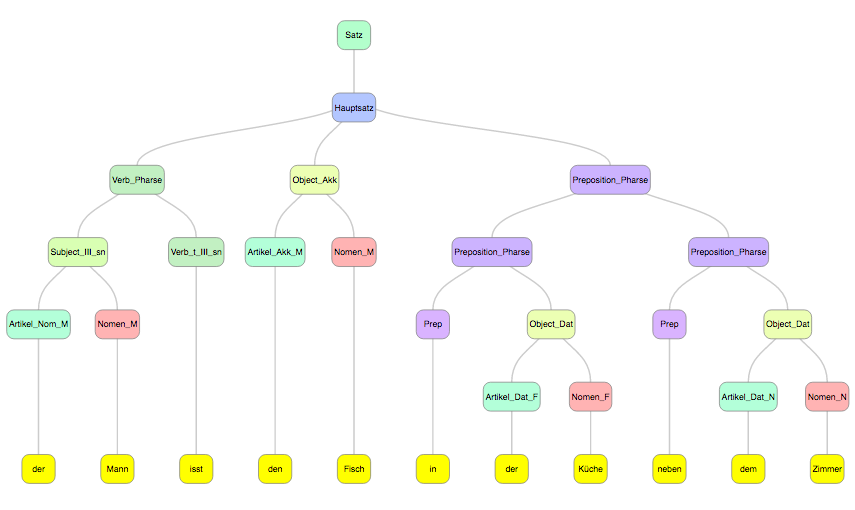
\includegraphics[scale=0.4]{onlineDemo}
\caption{Online Demo s použitím earley-parser-js}
  \label{fig:demo}
\end{figure}

\section{Prehľad technológií a nástrojov}

\subsection{Javascript}
Ako programovací jazyk pre túto aplikáciu budem používať Javascript. Je to dynamický, netypovaný, interpretovaný, vyšší programovací jazyk. Je veľmi vhodný pre tvorbu webových aplikácií, keďže je podporovaný všetkými modernými webovými prehliadačmi. Jazyk tiež zahŕňa API pre prácu s textom, poľami a regulárnymi výrazmi.

Pri písaní tejto aplikácie budem využívať aktuálnu špecifikáciu ECMAScript 6(2015), ktorú využíva Javascript. Pri použití tejto špecifikácie zároveň nehrozia problémy s kompatibilitou s webovými prehliadačmi, keďže, aplikácia bude fungovať na strane servera.\cite{js}

\subsubsection{Node.JS}
Node.js je Javascriptový runtime enviroment postavený na V8 Javascript engine od Google, vhodný pre tvorbu server-side aplikácií. Node.js využíva udalosťami riadený, asynchrónny model, ktorý ho robí veľmi rýchlym.


\subsection{JSON formát}
JSON je dátová štruktúra, respektíve formát, využívajúci pre človeka ľahko čitateľný text(štruktúru) skladajúci sa z dvojíc kľúč-hodnota. Jeho čitateľnosť ho robí veľmi výhodným napríklad pri uchovávaní gramatiky alebo slovníku pre našu aplikáciu, ktorá by mala byť dostatočne zrozumiteľná na to aby sa dala ľahko upravovať.


\subsection{XML}
XML je značkovací jazyk, ktorý je primárne určený na výmenu údajov medzi aplikáciami a na zverejňovanie dokumentov. Jazyk umožňuje opísať štruktúru dokumentu z hľadiska vecného obsahu jednotlivých častí. Sila XML je najmä v jeho hierarchickej štruktúre a pomerne jednoduchom spôsobe zápisu. Jazyk XML zároveň neobsahuje žiadne preddefinované tagy, teda užívateľ si ich definuje podľa vlastnej potreby, teda v našom prípade napríklad sentence a word tagy. XML dokument bude výstupom výslednej aplikácie.

%\subsection{Unit testy}
%\subsubsection{Jasmine}

%\subsubsection{Karma}

\chapter{Návrh a implementácia}
Táto časť práce bude venovaná návrhu a implementácii samotnej aplikácie. V podkapitolách sa najprv pristavím pri návrhu danej časti aplikácie a následne pomocou ukážok zdrojového kódu popíšem aj implementáciu.

\section{Perzistentné dáta}
Aplikácia nebude obsahovať vlastnú databázu, keďže bude modulom Multimediálnej čítanky, ktorá databázu má. Dáta(výstupy) aplikácie sa teda budú ukladať priamo do databázy Multimediálnej čítanky.

\section{Vstupné a výstupné dáta}
Vstupom pre aplikáciu bude reťazec v slovenskom alebo anglickom jazyku obsahujúci HTML formátovacie tagy(napr.: \verb@<b>, <i>, <span>@) a paragrafové tagy. Očakávaná dĺžka tohoto reťazca je maximálne okolo 1000 slov.

Výstupom bude XML reťazec, v ktorom budú tagmi označené jednotlivé slová a vety, s tým, že sa zachovajú všetky pôvodné HTML tagy zo vstupu bez toho, aby sa prekrížili s pridanými XML tagmi. Interpunkcia sa bude nachádzať mimo slovných tagov, pokiaľ teda nie je súčasťou slova. Príklad vstupu aj výstupu je možné vidieť v listingu (\ref{lst:vstup}) a (\ref{lst:vystup})
\begin{itemize}
\item formát vetného XML tagu: \verb@<s id="s\d+"></s>@
\item formát slovného XML tagu: \verb@<w id="w\d+"></w>@
\end{itemize}

Výstupom bude takisto aj parsovací strom použitý pre vytvorenie XML výstupu. Tento strom bude vo formáte JSON, kde každý vrchol bude mať atribúty \verb@name@ a \verb@children@. Prvý z nich bude buď menom gramatického pravidla alebo v prípade listov stromu to bude samotné slovo/interpunkcia a druhý bude poľom ďalších vrcholov s rovnakými atribútmi.

\section{Data-flow diagram}
\begin{figure}[h]
\centering
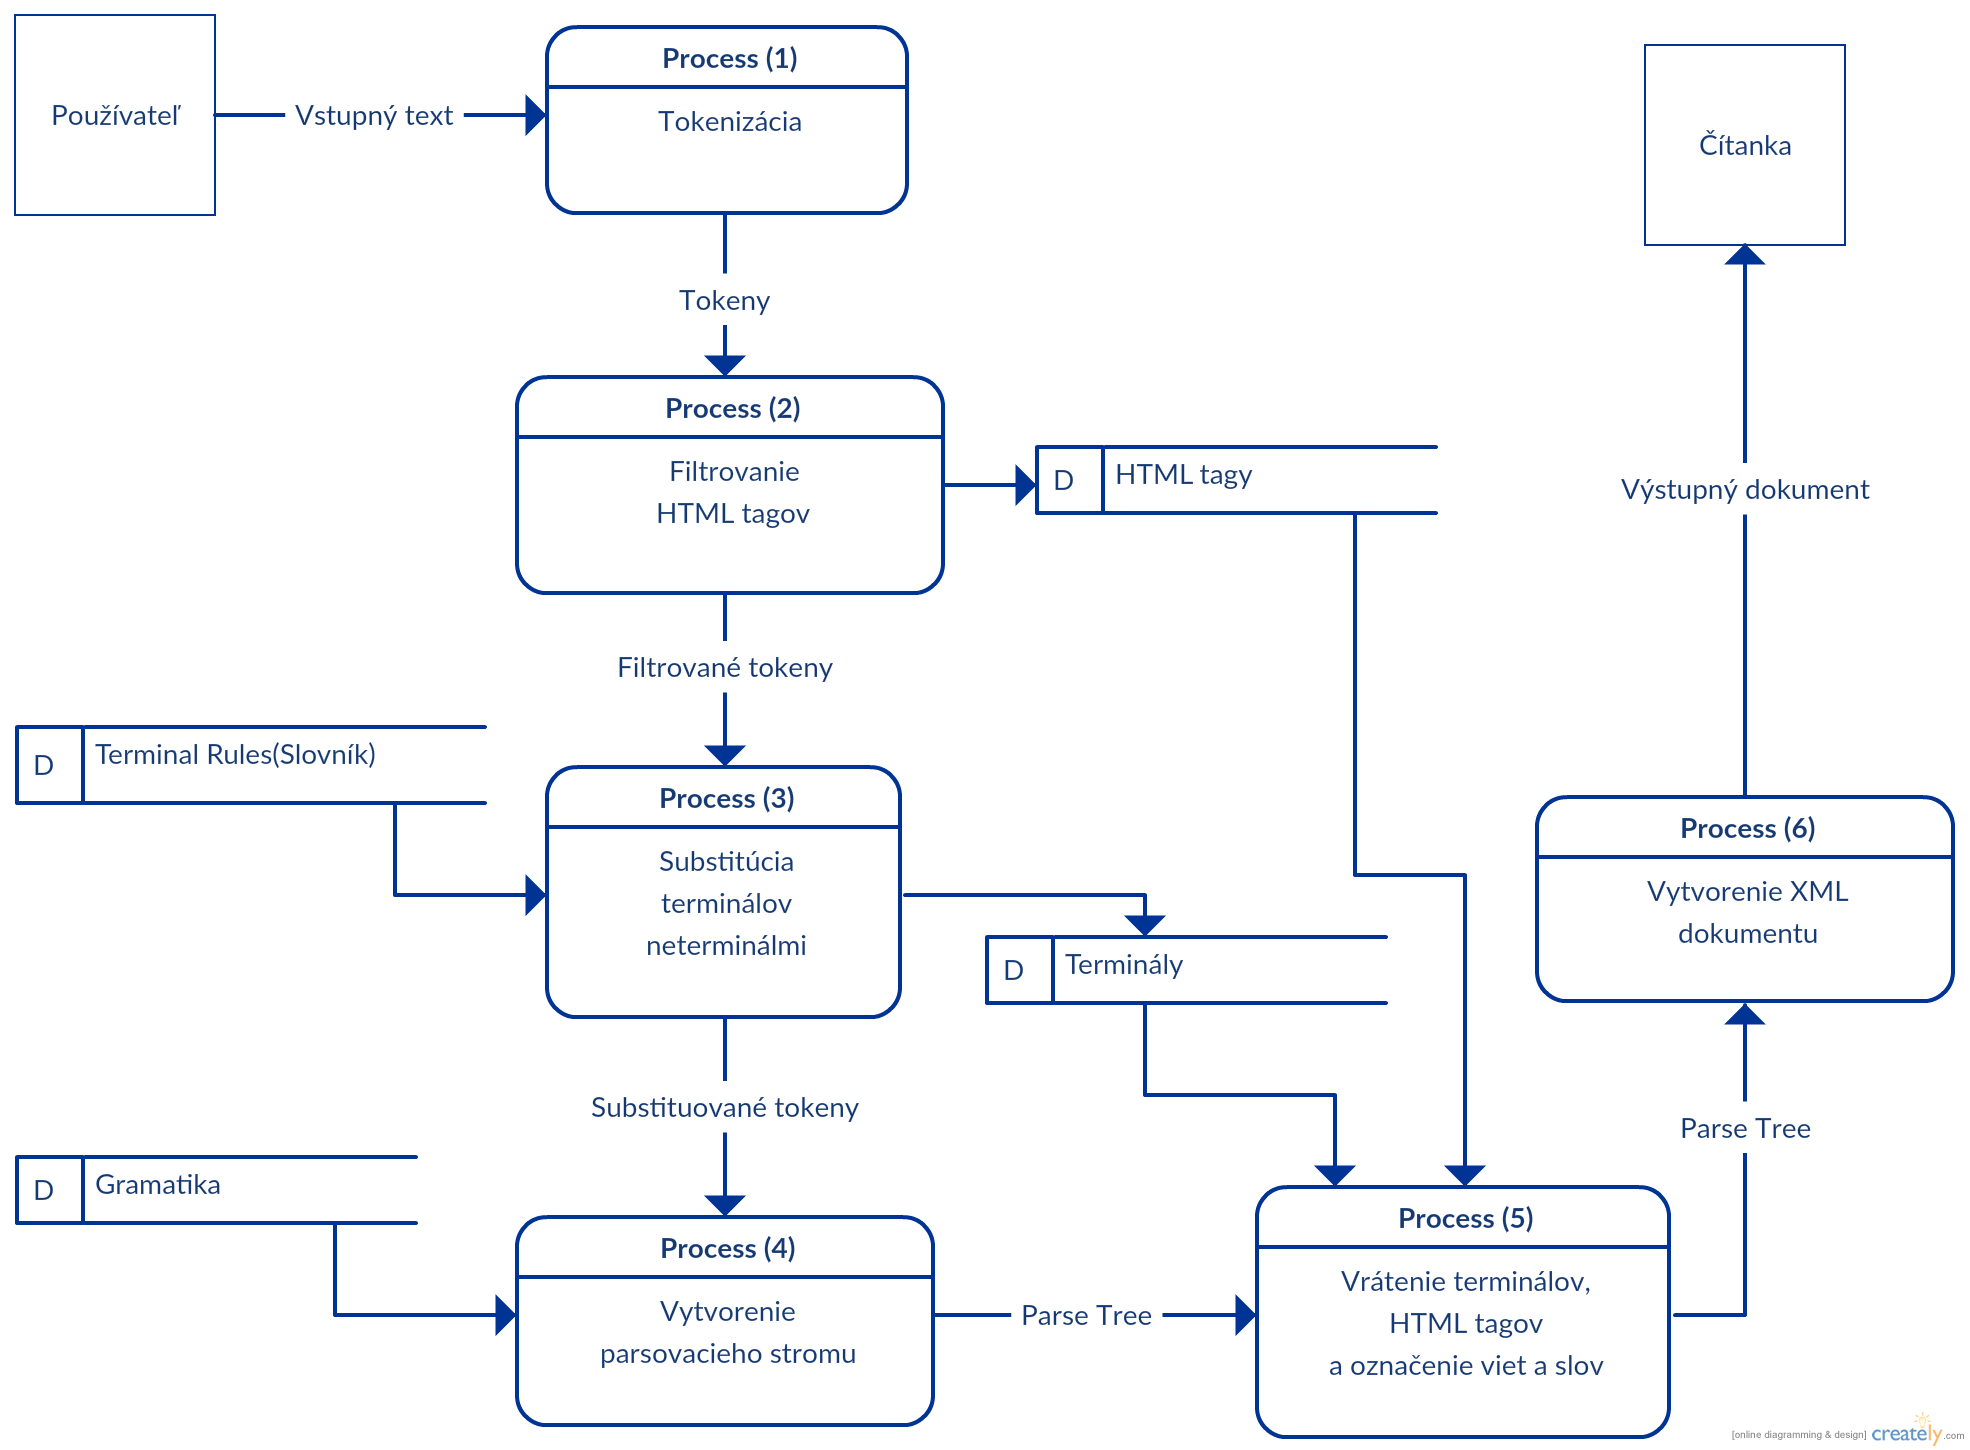
\includegraphics[scale=0.2]{DFD}
\caption{Data-Flow diagram}
  \label{fig:dataflow}
\end{figure}

Diagram(\ref{fig:dataflow}) popisuje tok dát a procesy v aplikácii. Na začiatku $(Process (1))$ aplikácia dostáva vstupný text od používateľa, ktorý sa pomocou regulárnych výrazov rozdelí na jednotlivé tokeny(slová, interpunkčné znamienka a pod.).

 Nasleduje proces filtrovania HTML tagov$(Process (2))$, kde sa z tokenov odstránia všetky HTML tagy a v tabuľke sa zapamätajú ich pozície, aby ich bolo možné neskôr vrátiť späť. 
 
Tieto filtrované tokeny je ďalej nutné nahradiť generickými tokenmi$(Process (3))$, (napr.: "dom" $\to  "Word"$), s ktorými sa bude ľahšie pracovať pri tvorbe gramatiky pre parser. Pôvodné tokeny sa samozrejme uložia, aby bolo možné neskôr zrekonštruovať pôvodný text. 

V tejto chvíli$(Process(4))$ prichádza na rad parser, ktorý pomocou gramatiky vytvorí parsovací strom zo substituovaných tokenov. 

Tento strom sa následne$(Process (5))$ upravý tak, že sa do listov vrátia pôvodné slová, pomocou štruktúry stromu sa označia jednotlivé slová a vety XML tagmi a pridajú sa HTML tagy na správne miesta. 

Nakoniec$(Process (6))$ sa z tohto finálneho stromu vytvorí XML dokument, ktorý dostáva Multimediálna čítanka na ďalšie spracovanie. V zbytku kapitoly presnejšie popíšem jednotlivé procesy zobrazené na diagrame.

\textit{Poznámka: Výsledná aplikácia implementuje možnosť používať slovenskú aj anglickú gramatiku(a aj slovník), tu sa však budem venovať hlavne tej slovenskej a len na miestach kde to bude potrebné spomeniem zmeny/rozdiely v anglickej.}
\section{Tokenizácia}
Text je nutné rozdeliť na tokeny, s ktorými sa bude dať ďalej pracovať. Tieto tokeny budú vytvorené pomocou regulárneho výrazu, ktorý rozdelí vstupný text na pole podreťazcov.
\noindent Typy tokenov, ktoré vzniknú:
\begin{itemize}
\item nové riadky - \verb@\n@
\item Opakujúca sa interpunkcia(napr.: ...(tri bodky), !?, !!!) - \verb|([\.!\?]{2,})|
\item triedy - \verb@([0-9]\.[A-Z])@ 
\item iniciály - \verb@([A-ZÉŘŔŤÝÚÍÓÁŠĎĹĽŽČ]\.)@
\item dátumy a časy vo formáte DD-MM-YYYY, HH:MM:SS,XXX \\ \verb@(\d{1,2}[:-]\d{1,2}[:-]\d{1,}(,\d+)*)@
\item čísla - \verb@([+-]?\d+(\.\d+)*(,\d+)?(%|,-)?)@ %(anglické radové číslovky) - % ([0-9]+(st|nd|rd|th))|(-?\d+(\.\d+)?)
\item bežné slová - keďže písmená so slovenskou diakritikou nepatria do rozsahov a-z prípadne A-Z, je nutné ich takýmto spôsobom vypísať - \\ \verb@((?!-)[a-zéŕřťýúíóášďľĺžčäôA-ZÉŘŔŤÝÚÍÓÁŠĎĹĽŽČ-]+)@
\item interpunkčné znamienka a ďalšie znaky - \verb@[\.,;:\"„“\(\)\?!'/\*\+%$€]@
\item HTML tagy - \verb@(<\s*\D*?>)@
\item znamineka menšie/väčšie - \verb@[<>]@ - tieto znamienka musia byť samostatne až za HTML tagmi, aby sa nestalo, že regex nájde samostatne len znamienka namiesto celých HTML tagov
\item všetko ostatné(non-whitespace) - \verb@[\S+]@
\end{itemize}

\noindent Výsledný regex je disjunkciou jednotlivých častí vyššie.


V tejto chvíli ešte nie je možné rozlíšiť napríklad radové číslovky("10.") , toto bude riešiť gramatika, ktorá bude "spájať" \ jednoduchšie tokeny dohromady($Ordinal \to Num $ $"."$).

\section{Filtrovanie HTML tagov}
V tokenoch vytvorených v predchádzajúcom kroku sa nachádzajú HTML tagy, ktoré chceme vo výslednom dokumente, ale pri parsovaní by nám iba prekážali, preto je potrebné ich dočasne vymazať, s tým, že si ich uložíme do pomocnej tabuľky v tvare:\\
\begin{lstlisting}[caption={Tabuľka HTML tagov}, style=htmlcssjs]
HTMLTagsPositions = {
		0:"<p>"
		4:"<i>"
		6:"</i>"
		9:"<b>"
		11:"</b>"
		14:"</p>"
		};
\end{lstlisting}

\noindent Kde kľúčmi sú indexy, na ktorých sa pôvodne nachádzali HTML tagy a hodnotami sú samotné tagy.

Zároveň sa z pôvodného poľa tokenov odstránia tieto tagy:
\begin{lstlisting}[caption={Text pred odstránením tagov}, style=htmlcssjs]
["<p>", "Toto", "je", "jednoduchá", "<i>", "veta", "</i>", "s",   "<b>", "html", "</b>", "tagmi", ".", "</p>"]
\end{lstlisting}
\begin{lstlisting}[caption={Text po odstránení tagov}, style=htmlcssjs]
["Toto", "je", "jednoduchá", "veta", "s", "html", "tagmi", "."]
\end{lstlisting}

\section{Substitúcia terminálov neterminálmi}
Keby sme chceli parseru poslať tokeny v takom stave v akom sú teraz, tak by sme na to potrebovali kompletný slovník, pomocou ktorého by parser vedel rozlíšiť, čo s ktorým slovom spraviť a zároveň by to tým pádom aj nafúklo gramatiku, ktorá by musela riešiť veľa zbytočných alternatív. Keďže hlbšia analýza slov a viet nie je cieľom tejto práce, tak  môžeme napríklad všetky slová s malými písmenami brať ako jeden typ tokenu($"WordLower"$).

Na tento účel použijeme tabuľku(slovník) pravidiel, ktorou prevedieme terminály na jednotlivé typy tokenov:\\
\newpage
\begin{lstlisting}[caption={Slovník s popisom},label={lst:label},style=htmlcssjs]
	{
	"^\n$": "NewLine", //Nové Riadky
	"^[0-9]\.[A-Z]$":"Class", //Trieda: napr. 1.A
	"^(prof|doc|Bc|Mgr|art|Mgr|Ing|Dr|[A-Z][A-Za-z]+Dr)$":
		"AcTitleBeforeName", //Tituly písané pred menom
	"^PhD$":"AcTitleAfterName", //Tituly písané za menom
	"^([A-ZÉŘŔŤÝÚÍÓÁŠĎĹĽŽČ]\.)$":"Initial", // Iniciály
	"^M{0,4}(CM|CD|D?C{0,3})(XC|XL|L?X{0,3})(IX|IV|V?I{0,3})$":
		"RomanNumeral", //Rímske číslice
	"^(č|t|j|r|tzv|tzn|napr|p|odb|str|písm|n)$":
		"StableTextAbbrStart", //Ustálené slovné skratky
	"^[a-zéŕřťýúíóášďľĺžčäô][a-zéŕřťýúíóášďľĺžčäô-]*
			[a-zéŕřťýúíóášďľĺžčäô]*$":"WordLower", //Slová s malými pís.
	"^[0-9]+$":"Num", //Čísla
	"^(\d{1,2}[:-]\d{1,2}[:-]\d{1,}(,\d+)*)|([+-]?\d+(\.\d+)*(,\d+)?(%|,-)?)$":"Decimal", //Desatinné čísla, dátumy a časy
	"^[\\.]{3,}$":"Ellipsis", //Tri(alebo viac) bodky
	"^[\.!\?]{2,}$":"RepeatedPunctuation", //Opakujúca sa interpunkcia
	"^\.$":".", //Bodka
	"^,$":",", //Čiarka
	"^;$":";", //Bodkočiarka
	"^\?$":"?", //Otáznik
	"^!$":"!", //Výkričník
	"^[-\u2014\u2013\u2212\u2010\u2011]$":"-", //Pomlčka
	"^:$":":", //Dvojbodka
	"^\"$":"\"", //Úvodzovky
	"\u201E": "\u201E", //Slovenské úvodzovky(dole)
	"\u201C": "\u201C", //Slovenské úvodzovky(hore)
	"^[A-ZÉŘŔŤÝÚÍÓÁŠĎĹĽŽČ][a-zéŕřťýúíóášďľĺžčäô-]*$":"WordCapital", //Slovo s veľkým začiatočným písmenom
	"^[A-ZÉŘŔŤÝÚÍÓÁŠĎĹĽŽČ]{2,}$":"WordAbbr", //Skratky(všetko veľké)
	"^[A-ZÉŘŔŤÝÚÍÓÁŠĎĹĽŽČa-zéŕřťýúíóášďľĺžčäô-]+$":"Word", //Ostatné slová
	"^\S+$": "Other" // ostatné tokeny(non-whitespace)
	};
\end{lstlisting}
		%"([0-9]+(st|nd|rd|th))":"Ordinal" //radove cislovky(anglicke)

\noindent Po tejto úprave môže veta vyzerať napríklad takto: \\
\begin{lstlisting}[caption={Tokeny po použití slovníku},style=htmlcssjs]
tokens = 
["WordStart",  "WordLower",  "Word", "-", "WordLower", "Decimal", "WordLower", "Word", "?"]
\end{lstlisting}

\section{Vytvorenie parsovacieho stromu}
Na vytvorenie parsovacie stromu bude použitý earley-parser-js, ten však potrebuje pre svoju prácu tokeny(popísané v predchádzajúcej podkapitole) a gramatiku. Gramatika bude vo forme poľa pravidiel, kde $"\to"$ označuje rozdelenie na ľavú a pravú stranu pravidla a $"\mid"$ označuje alternatívu(v tomto príklade je použitá gramatika na parsovanie jednoduchej aritmetiky):

\begin{lstlisting}[caption={Ukážková gramatika},label={lst:gramatika},style=htmlcssjs]
var grammar = new tinynlp.Grammar([
    'Root -> N',
    'S -> S add_sub M | M',
    'M -> M mul_div T | T',
    'N -> S lt_gt S | S',
    'T -> num | ( S )',
]);
\end{lstlisting}

\bigskip A pre terminály: 

\begin{lstlisting}[caption={Vytvorenie pravidiel pre terminály}, style=htmlcssjs]
grammar.terminalSymbols = function(token) {
    if ('<' === token || '>' === token) return ['lt_gt'];
    if ('+' === token || '-' === token) return ['add_sub'];
    if ('*' === token || '/' === token) return ['mul_div'];
    if ('(' === token) return ['('];
    if (')' === token) return [')'];
    // Otherwise - token considered as a number:
    return ['num'];
};
\end{lstlisting}

\bigskip Pri termináloch nám prácu uľahčí to, že už máme vytvorený slovník (Listing \ref{lst:label}), teda nebude nutné nijak nahrádzať tokeny, teda v našom prípade: \\
\begin{lstlisting}[style=htmlcssjs]
grammar.terminalSymbols = function(token) {
    return [token];
};
\end{lstlisting}
\bigskip
Na to, aby sme zabezpečili možnosť ľahko upravovať gramatiku, tak ju budeme mať uloženú v textovom súbore vo formáte JSON, kde atribútom bude ľavá strana pravidla a hodnotou bude pravá strana. Vyššie uvedená gramatika(Listing \ref{lst:gramatika}) by teda vyzerala takto:
\newpage
\begin{lstlisting}[caption={Ukážková gramatika V JSON-e},label={lst:gramatikaJSON},style=htmlcssjs]
{
	"Root":"N",
	"S":"S add_sub M | M",
	"M":"M mul_div T | T",
	"N":"S lt_gt S | S",
	"T":"num | ( S )"
}
\end{lstlisting}

A tým pádom načítavanie gramatiky bude zjednodušené: \\

\begin{lstlisting}[style=htmlcssjs]
var grammar = new tinynlp.Grammar(this.loadGrammar(rulePath));
\end{lstlisting}

\subsection{Analýza gramatiky}
%TODO: ked bude hotova gram., tak rozobrat jednotlive pravidla.

Koreňom celej gramatiky je $"Story"$, z ktorého sa v prípade slovenskej gramatiky vetvia jednotlivé riadky, teda: $$"Story \to Lines "$$  V anglickej gramatike sú to jednotlivé vety: $$"Story \to Sentences "$$

Tento rozdiel je spôsobený tým, že v Slovenčine sa používa priama reč vymedzená pomlčkami a tam sa zvyknú dávať jednotlivé súvetia, respektíve prehovor jednej osoby, do samostatných riadkov, teda vedieť kde končí riadok je veľmi užitočné, napríklad: \\

\noindent - Prídeš? - spýtal sa Jožko.\\
- Prídem...\\
- Určite? - spýtal sa znova. Lebo si nebol istý...\\
- Určite! \\

My nevieme vopred koľko viet/riadkov bude v texte, tým pádom pravidlo pre vety/riadky musí byť rekurzívne: $$"Sentences \to Sentences \ Sentence \ | \ Sentence"$$  $$"Lines \to Lines \ Line \ | \ Line"$$
Tieto pravidlá sa môžu zdať neprirodzene zapísané(najprv rekurzívny prípad, až potom triviálny). Dôvodom je, že tento parser má lepší výkon pri $"left-recursive"$\  gramatike(testy gramatiky v \hyperref[tests]{kapitole \ref{tests}}) a tiež je to potrebné pri pridávaní \verb!<p>! tagov, ktoré by pri $"right-recursive"$ \ gramatike mohli skončiť na nesprávnom mieste, kvôli tomu, že to zmení ich najbližšieho spoločného parenta, napríklad:
\begin{figure}[H]

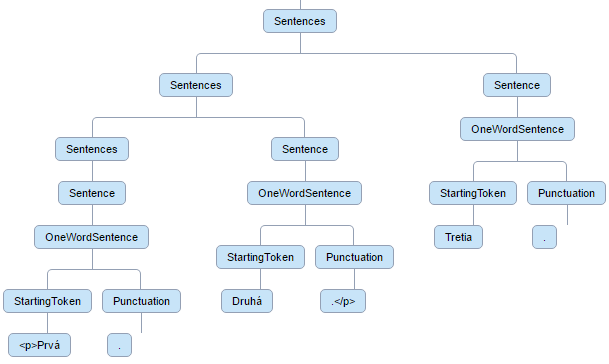
\includegraphics[scale=2.4]{treePTagsCorrect}
\caption{Správny výstup pre vstup: \texttt{<p>Prvá. Druhá.</p> Tretia.}}
\end{figure}
\begin{figure}[H]
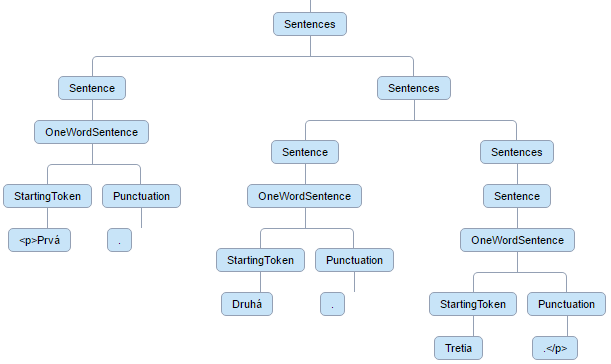
\includegraphics[scale=2.4]{treePTagsIncorrect}
\caption{Nesprávny výstup pri $"right-recursive"$ gramatike}
\end{figure}

\textit{Poznámka: Všetky ukážky stromov sú zjednodušené kvôli čitateľnosti a kompaktnosti.}
\textit{Keďže v ostatných pravidlách sa poväčšine anglická a slovenská gramatika líšia v štruktúre a nie veľmi v zmysle, tak budem popisovať iba tú slovenskú, keďže je pre nás relevantnejšia.} 

Ďaľším pravidlom je $"Line"$, ktorý rozlišuje medzi dvomi typmi viet a logicky končí novými riadkami(aspoň jedným):
$$"Line \to \ DirectSpeechDashStart \ NewLines \ | \ OtherSentences \ NewLines "$$

\noindent $"DirectSpeechDashStart"$ je skupinou pravidiel, ktoré definujú priamu reč vymedzenú pomlčkami a $"OtherSentences"$ združujú priamu reč v úvodzovkách a ostatné jednoduché vety. Najprv sa pozrieme na jednoduché vety a následne na priame reči: \\


\noindent Najjednoduchšou formou vety je $"Sentence"$ z nej môže vzniknúť \\ $"OneWordSentence"$ alebo $"BasicSentence"$
\begin{itemize}
\item $"OneWordSentence"$ sa musí skladať z $"StartingToken"$ a $"Punctuation"$, kde prvý z nich je slovom s veľkým začiatočným písmenom, číslom alebo iným tokenom, ktorým môže začínať veta a druhým je interpunkcia, ktorá môže ukončovať vetu - napríklad: bodka, otáznik, tri bodky, ale nie čiarka.
\item $"BasicSentence"$ je vo forme: $"StartingToken \ \ Words \ Punctuation \ | \ Quotation"$
	rozdielom oproti $"OneWordSentence"$ sú ďalšie slová, ktoré sú definované podobne ako $"Sentences"$ alebo $"Lines"$(rekurzívne) a alternatíva v podobe vety s citátom, ktorá obsahuje navyše aj ľavé a pravé úvodzovky, ktoré však neoznačujú priamu reč, teda nie sú samostatnou vetou.
\end{itemize}

Ďalej gramatika popisuje už spomínané typy priamej reči. V Slovenčine poznáme priamu reč s úvodzovkami  alebo pomlčkami. Tá s úvodzovkami má štyri formy:
\begin{enumerate}[leftmargin=*]
\item „Priama reč\verb@[.?!]+@“
\item Uvádzacia veta: „Priama reč\verb@[.?!]+@“
\item „Priama reč\verb@[,?!]+@“ uvádzacia veta\verb@[.?!]+@
\item „Priama reč\verb@[,?!]+@“ uvádzacia veta, „priama reč\verb@[.?!]+@“
\end{enumerate}

\textit{Poznámka: Priama reč a Uvádzacia veta tu neoznačujú jednu vetu, ale ľubovoľný počet viet, posledná z nich však musí končiť jedným zo znamienok popísaných regulárnym výrazom.}

\begin{enumerate}[leftmargin=*]
\item Prvá možnosť je definovaná pomocou troch pravidiel:$"DirectSpeechSingle"$,  \\$"DirectSpeechTwo"$ a $"DirectSpeechMoreThanTwo"$
Toto rozdelenie je potrebné, aby sme vedeli dať začiatočné a koncové úvodzovky do správnej vety. V prvom prípade, teda aj začiatočné aj koncové úvodzovky patria do jednej vety, v druhom prípade začiatočné do prvej a koncové do druhej a v treťom prípade začiatočné do prvej, koncové do poslednej a medzi nimi sa nachádza ľubovoľný počet $"Sentences"$.


\noindent Samotné pravidlá:
\begin{itemize}
\item $"DirectSpeechSingle \to \\
QuoteLeft \ StartingToken \ Punctuation \ QuoteRight \ |\\ QuoteLeft \ StartingToken \ Words \ Punctuation \ QuoteRight"$
\item $"DirectSpeechTwo \to DirectSpeechFirst \ DirectSpeechSecond"$
\item $"DirectSpeechMoreThanTwo \to \\ DirectSpeechFirst \ Sentences \ DirectSpeechSecond"$
\end{itemize}
 $"DirectSpeechFirst"$ a $" DirectSpeechSecond"$ vyzerá takmer rovnako ako \\ $"DirectSpeechSingle"$, jediným rozdielom je absencia začiatočnej respektíve koncovej úvodzovky.
\item Pre vytvorenie pravidiel pre ostatné typy priamej reči potrebujeme zadefinovať ako budú vyzerať uvádzacie vety, kde v prípade uvádzacej vety na začiatku to bude:
$"ISentenceStart \to StartingToken \ Words : | \ StartingToken :"$ \\ Za ktorou bude nasledovať jedna z priamych rečí z predchádzajúceho bodu.

\textit{Poznámka: DS = Direct Speech, IS = Introductory Sentence}

\item Tretia možnosť nás núti upraviť priamu reč aj uvádzaciu vetu z predchádzajúcich prípadov:
	\begin{itemize}
	\item Priama reč teraz nemôže končiť bodkou, teda namiesto $"Punctuation"$  použijeme $"DSPunctuation \to \ , | \ ? \ | \ ! \  | \ RepeatedPunctuation \ | \ Ellipsis"$, inak táto priama reč ostáva rovnaká ako to bolo v prvom prípade.
	\item Uvádzacia veta zase môže začínať aj malým písmenom, tým pádom bude vo forme: $"ISentenceEnd \to \ Words \ Punctuation"$
	\end{itemize}
Výsledné pravidlo:$"DSAndISentence \to \ DirectSpeechStart \ ISentenceEnd"$

\item Pri poslednom prípade si treba uvedomiť, že druhá a tretia časť vety sa môže ľubovoľne opakovať, napr.: 

\verb@...uvádzacia veta,„priama reč[,?!]+@“ \verb@uvádzacia veta,„priama reč[.?!]+@“


teda druhá(opakujúca sa) časť vety potrebuje rekurzívnu definíciu. Celá veta:


$"DSAndISentenceRepeated \to \ DirectSpeechStart \ ISAndDSRepeated"$

Rekurzívna definícia:


$"ISAndDSRepeated \to \\ ISAndDSRepeated \ ISentenceMiddle \ DirectSpeechEnd \ | \\ \ ISentenceMiddle\ DirectSpeechEnd"$

kde $"ISentenceMiddle"$ sa skladá z viacerých viet s tým, že prvá môže začínať malým písmenom a posledná z nich musí končiť čiarkou. Medzi nimi sa môžu nachádzať $"Sentences"$ 
\end{enumerate}
\newpage
\noindent S pomlčkami:
\begin{enumerate}[leftmargin=*]
\item - Priama reč\verb@[.?!]+@
\item - Priama reč\verb@[,?!]+@ - uvádzacia veta\verb@[.?!]+@
\item Uvádzacia veta: - Priama reč\verb@[.?!]+@“
\item - Priama reč\verb@[,?!]+@ - uvádzacia veta\verb@[,?!]+@ - priama reč\verb@[.?!]+@
\end{enumerate}

\begin{enumerate}[leftmargin=*]
\item Tu v prvom prípade vieme vytvoriť priamu reč jednoduchším spôsobom, keďže nemusíme riešiť úvodzovky na začiatku aj na konci, ale len pomlčku na začiatku. Na tomto mieste tiež využijeme to, že náš text sa delí na riadky ukončené \verb!\n! - teda, žiadna z viet, z ktorých sa skladá toto pravidlo nebude ukončená novým riadkom a ak sa v texte vyskytne medzi takýmito vetami nový riadok, tak sa o to postará pravidlo $"Line"$.

$"DirectSpeechDash \\ \to \ SentenceDashNoNewLines \ \ SentencesNoNewLine \ \ |  \ \ SentenceDash"$
\item V druhom prípade vytvoríme pravidlo z dvoch častí:

$"DSAndISentenceDash \to \ DirectSpeechStartDash \ ISentenceEndDash"$ 


kde prvou časťou je priama reč($"DirectSpeechStartDash"$). Toto pravidlo je rozdelené podobne ako prvá možnosť pri priamej reči s úvodzovkami. Tu toto rozdelenie ale potrebujeme kvôli tomu, aby sme vedeli, v ktorej vete bude začiatočná pomlčka, ktorá bude v klasickej forme a ktorá nemôže končiť bodkou. Druhá časť($"ISentenceEndDash"$) pravidla zase začína pomlčkou a môže mať prvé slovo s malým písmenom.
\item Ďalšia možnosť je len spojením uvádzacej vety($ISentenceStart$), ktorú sme použili pri priamej reči s úvodzovkami a priamej reči s pomlčkou z prvého bodu:


$"ISentenceAndDSDash \to \ ISentenceStart \ DirectSpeechDash"$
\item Poslednou možnosťou ako poskladať priamu reč s pomlčkami je použiť priamu reč na začiatku, ktorú sme už spomínali vyššie($"DirectSpeechStartDash"$) a za ňou, pridať ďalšie dve časti, kde prvá je uvádzacou vetou v podobnej forme ako tomu bolo v 2. bode, s tým rozdielom, že tu nemôže táto uvádzacia veta končiť bodkou. Poslednou časťou je priama reč, ktorá rovnako ako predchádzajúca časť môže začínať malým písmenom, nemôže však končiť čiarkou, keďže je to koniec vety:


$"DSAndISentenceDashRepeated \to 
\\ DirectSpeechStartDash \ \ ISentenceMiddleDash\ \ DirectSpeechEndDash"$


%kde druhá časť bude vyzerať:
%
%
%$"ISAndDSDashRepeated \to \ ISentenceMiddleDash\ DirectSpeechEndDash"$
\end{enumerate} 

Tak ako už bolo spomenuté vyššie tak v Angličtine sa priama reč určená pomlčkami nepoužíva, takže v tomto ohľade je trochu jednoduchšia. V Angličtine sa ale používajú rôzne typy úvodzoviek na určenie priamej reči, tam teda musia byť využité tieto tri typy namiesto slovenských úvodzoviek:

$$InvertedComa \to "\text{`}", \ InvertedDoubleComa \to"\text{``}", \  Quote \to """$$

\subsubsection{Optimalizácia}
Kvôli skutočnosti, že v Slovenčine môžeme skombinovať takmer hocijakú postupnosť slov a interpunkcie a aj tak vytvoriť valídnu vetu, tak by pre nás bolo najjednoduchšie definovať slová vo vete ako hocijaké slová, interpunkciu a nové riadky. To ale spôsobí veľmi veľké množstvo nejednoznačností v gramatike a parser bude produkovať veľmi veľa zbytočných stromov. Tieto nejednoznačnosti primárne spôsobuje priama reč určená pomlčkami, v ktorej sa za sebou vyskytujú interpunkčné znamienka, ktoré môže obsahovať aj jednoduchá slovenská veta, v tej by sa však nemali objaviť hneď za sebou.
\begin{lstlisting}[caption={Nejednoznačný vstup},style=htmlcssjs]
- Priama reč, - uvádzacia veta, - Priama reč...
\end{lstlisting}
\begin{lstlisting}[caption={Výstupné vety vo forme polí},style=htmlcssjs, label={lst:opt}]

[["-", "Priama", "reč", ","],
 ["-", "uvádzacia", "veta"],
 ["-", "Priama", "reč", "."]] // korektný výstup
 
 ["-", "Priama", "reč", ",", "-", "uvádzacia", "veta", "-", "Priama", "reč", "."] // jeden z nekorektných výstupov
\end{lstlisting}
Ako môžeme vidieť v listingu (\ref{lst:opt}) parser nemusí nutne rozoznať čiarku a pomlčku ako koniec a začiatok priamej reči. Preto potrebujeme kombinácie niektorých interpunkčných znamienok vylúčiť z gramatiky. CFG však nepozná negácie, preto v tejto situácii zadefinujeme slová ako dve alternatívy. Prvou z nich je, že slovo bude samostatne a druhou, že slovo bude vo dvojici s našou nechcenou interpunkciou, to zamedzí tomu, aby sa priamo za sebou v bežných vetách vyskytla napríklad čiarka a pomlčka.
$$"MidSentencePunctuation \to \ , \ | \ ; \ | \ : \ | \ Dash \  | \ Ellipsis"$$
$$"WordBasic \to  \ WordCapital \ | \ WordLower \ | \ Initial \ | \ Word \ | \ Number ..."$$
$$"WordTokens  \to\  WordBasic \ | \ WordBasic \ MidSentencePunctuation"$$

\newpage
Táto podkapitola samozrejme neobsahuje všetky pravidlá, ktoré sa nachádzajú v gramatike, preto odporúčam pre ďalšie podrobnosti ohľadne gramatiky pozrieť si samotné zdrojové súbory gramatiky, ktoré sa nachádzajú v prílohách v zdrojových súboroch v priečinku: \verb@parser/app/res/grammars@, prípadne využiť priloženú vizualizáciu.


\subsection{Parsovací strom}
Earley-parser-js vráti ako výstup parsovací strom, ktorý je v JSON formáte, kde atribútmi sú $"root"$(koreň) podstromu(ľavá strana pravidla, ktoré sa začína v danom vrchole), $"left"$(začiatok, respektíve index tokenu pred ktorým pravidlo začalo), $"right"$(koniec, respektíve index tokenu, za ktorým končí toto pravidlo) a $"subtrees"$ \\ (podstromy, respektíve potomkovia tohto vrcholu). Napríklad: 
\begin{lstlisting}[style=htmlcssjs, basicstyle=\fontsize{9}{11}\ttfamily]
 {
 	...
	"root": "SentenceSimple",
		"left": 6,
		"right": 8,
		 "subtrees": [{
			"root": "OneWordSentence",
			"left": 6,
			"right": 8,
			"subtrees": [{
				"root": "StartingToken",
				"left": 6,
				"right": 7,
				"subtrees": [{
					"root": "<s id="s2"><w id="w5">Veta</w>",
					"left": 6,
					"right": 7,
					"subtrees": []
				}]
			},
			{ ... }]}]}]}]}
\end{lstlisting}

%			"root": "Punctuation",
%			"left": 7,
%			"right": 8,
%			"subtrees": [{
%				"root": ".</s>",
%				"left": 7,
%				"right": 8,
%				"subtrees": []



\subsection{Neúplný pars}
V prípade, že by sa parseru nepodarilo získať zo vstupu úplný pars(vo vstupe je chyba), tak je earley-parser-js upravený tak, aby vrátil strom zahŕňajúci najdlhší čiastočný pars textu, ktorý začína na začiatku vstupného textu. Pre zachovanie štruktúry stromu sa ostávajúci nesparsovaný text spojí do jednej vety. Všetky ostatné tagy sa umiestnia, tak ako pri úplnom parse.

Toto riešenie by malo pomôcť užívateľovi ľahšie si nájsť chybu vo svojom texte, keďže je zjavné, od ktorej vety už text nie je rozdelený a chyba by prirodzene mala byť niekde na začiatku tejto vety(napríklad malé písmeno na začiatku vety).

\section{Vrátenie terminálov}

V tejto chvíli už máme k dispozícii všetko potrebné na vybudovanie výsledného XML. Ako prvé je potrebné vrátiť do stromu - ktorý nám vytvoril parser - tokeny(slová a interpunkciu), lebo ak by sme najprv pridávali všetky tagy, tak by sme zbytočne museli riešiť, ktorú časť hodnoty daného vrcholu stromu treba nahradiť.

Keďže jednotlivé listy stromu sú v tom istom poradí, ako boli tokeny, ktoré vznikli po odstránení HTML tagov, tak nám stačí prejsť všetky listy a v tomto istom poradí ich nahradiť:

%\begin{lstlisting}[style=htmlcssjs]
%substituteLeafs(tree = this.tree) {
%	if (tree.subtrees.length == 0) {
%		tree.root = this.tokenizer.originalTokens[tree.right - 1];
%	}
%	else {
%		for (let node of tree.subtrees) {
%			this.substituteLeafs(node);
%		}
%	}
%}
%\end{lstlisting}

%TODO: pridat obrazok HTML stromu.
\begin{figure}[h]
\centering
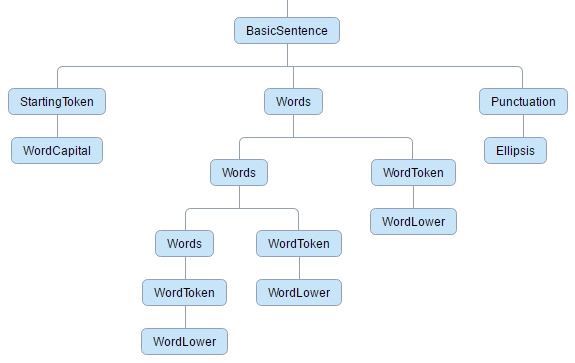
\includegraphics[scale=2.6]{treeBeforeSubstitution}
\caption{Strom bez terminálov}
\end{figure}

\begin{figure}[H]
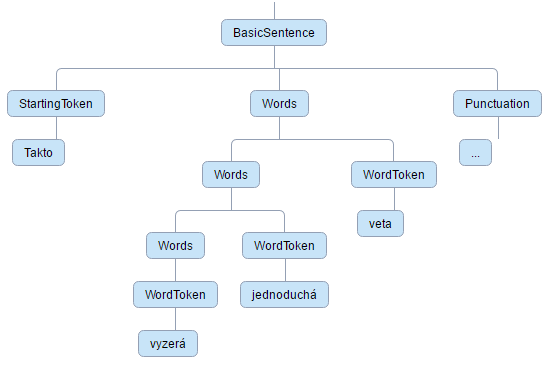
\includegraphics[scale=2.4]{treeAfterSubstitution}
\caption{Strom po substitúcii}
\end{figure}

\section{Označenie slov a viet}
\subsection{Označenie slov}
Pri pridávaní $"Word"$ tagov je potrebné si dať pozor na tokeny, ktoré sú rozdelené do viacerých listov, napríklad: $"Ordinal \to Num $ $ "." \ "$. Tieto "slová"  \ síce nie sú v jednom vrchole, ale aj tak ich chceme označiť jedným tagom.

Vďaka štruktúre stromu vieme povedať, že to čo chceme obaliť $"Word"$ tagom, sú všetky listy prislúchajúce jednému priamemu rodičovi. Teda ak sú všetci potomkovia vrcholu listy a aspoň jeden z nich nie je interpunkcia, tak prvému z týchto listov dáme otvárací tag a poslednému uzatvárací(vo väčšine prípadov je to len jeden vrchol).

%\begin{lstlisting}[style=htmlcssjs]
%addWordTags() {
%	var counter = 1;
%	function add(self, tree) {
%		if (tree.subtrees.every(Parser.isLeaf) && !tree.subtrees.every(self.isPunctuation, self)) {
%			tree.subtrees[0].root = '<w id="w'+ counter +'">' + tree.subtrees[0].root;
%			tree.subtrees[tree.subtrees.length - 1].root += '</w>';
%			counter += 1;
%		 } else {
%		 	for (let node of tree.subtrees) {
%		 		add(self, node);
%			}
%		}
%	}
%	add(this, this.tree);
%}
%\end{lstlisting}

Ak list obsahuje iba interpunkciu, tak ho vynechávame, lebo nás v tejto chvíli zaujímajú len slová.

\begin{figure}[H]
\centering
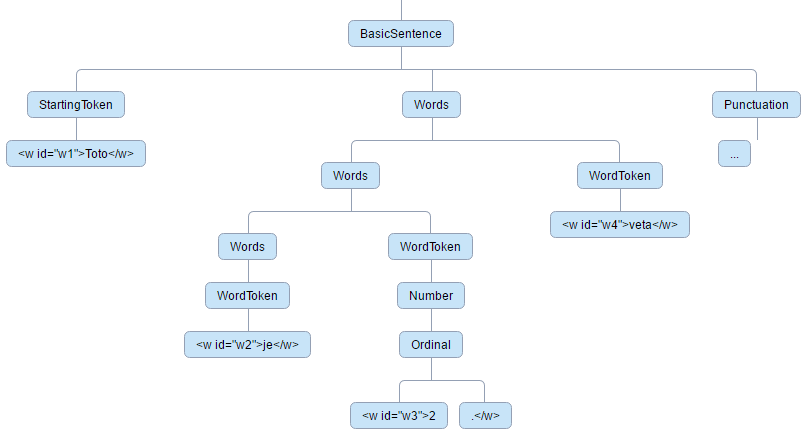
\includegraphics[scale=2.2]{treeWordsAdded}
\caption{Strom s \textit{"Word"} tagmi}
\end{figure}


\subsection{Označenie viet}
Na to, aby sme mohli pridávať do textu \verb@<s>@ tagy, potrebujeme vedieť, ktoré pravidlá gramatiky označujú vety, napríklad: $$"BasicSentence": "StartingToken\ Words\ Punctuation\ |\ Quotation"$$ Preto v konfigurácii pre každú gramatiku je zadefinované pole $"SentenceRule"$, ktoré je poľom všetkých pravidiel gramatiky, ktoré by mali mať vo výslednom texte tento tag.

\begin{lstlisting}[style=htmlcssjs]
"sentenceRule": ["ISentenceStart", "ISentenceEnd", "DirectSpeechDash", "OneWordSentence", "BasicSentence",         "Sentence", "DirectSpeechSingle",  ...]
\end{lstlisting}

Tieto tagy, teda pridávame vždy najľavejšiemu(otvárací) a najpravejšiemu(uzatvárací) vrcholu daného podstromu, ktorého koreňom je vrchol s jedným s vyššie uvedených pravidiel.
\begin{lstlisting}[style=htmlcssjs]
addSentenceTags(tree = this.tree) {
	var counter = 1;
	function add(self, t) {
		if (t != undefined) {
			for (let node of t.subtrees) {
				if (self.config["sentenceRule"].includes(node.root)) {
					if (self.checkParent(tree, node)) {
						self.addOpeningSentenceTag(node, counter);
						self.addClosingSentenceTag(node);
						counter++;
					}
				}
				add(self, node);
			}
		}
	}
	add(this, this.tree);
}
\end{lstlisting}

Funkcia sa volá na každý vrchol parsovacieho stromu vrátane vrcholov podstromu, ktorý už bol označený \verb@<s>@ tagom, keďže vety v texte sa môžu vnárať jedna do druhej. Funkcia zároveň zabezpečuje, že všetky tagy budú v správnom poradí, teda že na vrchu bude vždy tag s najmenším poradovým číslom.

\begin{figure}[H]
\centering
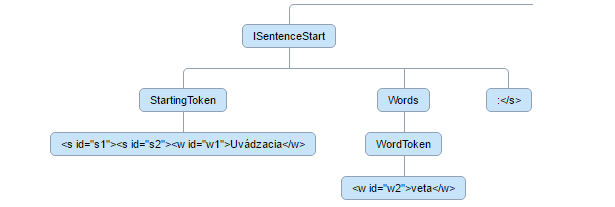
\includegraphics[scale=2.8]{sentenceTagsAndNestedSentenceLeft}
\caption{Strom s \texttt{<s>}  tagmi a vnorenou vetou(ľavá strana)}
\end{figure}
\begin{figure}[H]
\centering
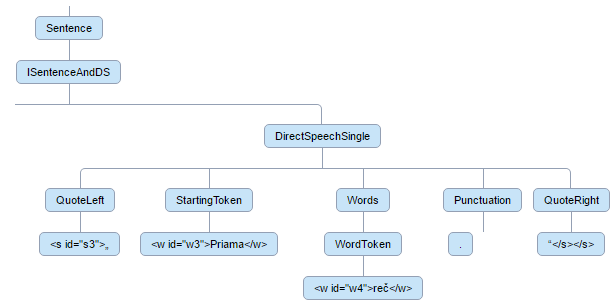
\includegraphics[scale=2.6]{sentenceTagsAndNestedSentenceRight}
\caption{Strom s \texttt{<s>}  tagmi a vnorenou vetou(pravá strana)}
\end{figure}

\section{Vrátenie HTML tagov}
Pri HTML tagoch rozlišujeme formátovacie tagy(\verb!<b>, <i>, <span>...!) a paragrafy (\verb!<p> </p>!). Paragrafy by sa po správnosti nemali nachádzať vnútri viet, na to sa však nedá plne spoliehať. Keby sa vyskytla takáto chyba v texte, spôsobilo by to, že by sa prekrížili \verb@<s>@ tagy s tými paragrafovými, preto je potrebné skontrolovať a prípadne posunúť paragrafové tagy na začiatok, respektíve na koniec vety, v ktorej sa nachádzajú.
\begin{figure}[H]
\centering
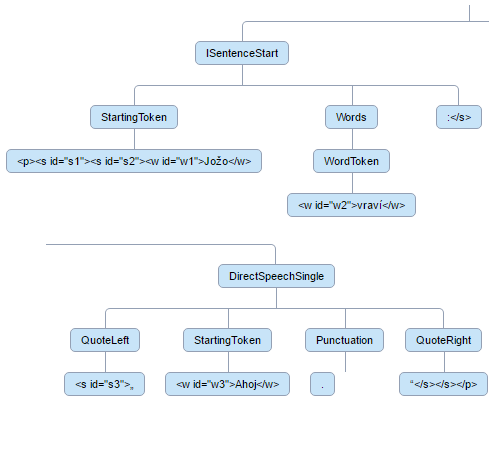
\includegraphics[scale=2.6]{adjustedPTags}
\captionsetup{width=.7\linewidth}
\caption{Príklad stromu s posunutým \texttt{<p>} tagom pre vstup: \texttt{\char`\"Jožo <p>vraví: \char`\"</p>Ahoj.\char`\"\char`\"}}
\end{figure}

Pokiaľ ide o formátovacie tagy, tie môžu zahŕňať jedno slovo, jednu vetu alebo kľudne môžu aj začínať v strede jednej a končiť v strede druhej. Formátovacie tagy, ale na rozdiel od tých paragrafových vieme rozdeliť na časti, tak aby sa zabránilo kríženiu. Ak teda tag prechádza cez hranice viet, tak ho na konci prvej uzatvoríme a na začiatku ďalšej zase otvoríme.
\begin{figure}[H]
\centering
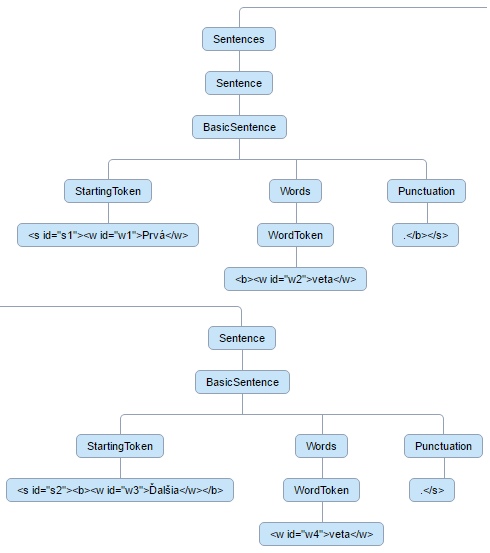
\includegraphics[scale=2.6]{dividedFormattingTags}
\captionsetup{width=.7\linewidth}
\caption{Príklad stromu s rozdeleným \texttt{<b>} tagom pri vstupe: \texttt{\char`\"<p>Prvá <b>veta. Ďalšia</b> veta.</p>\char`\"}}
\end{figure}

\section{Vytvorenie XML dokumentu}
Po všetkých predchádzajúcich krokoch už máme v listoch stromu kompletný text so všetkými tagmi, ktoré chceme, teda nám už len stačí spojiť hodnoty jednotlivých listov dohromady a tým vznikne výsledný text.

\chapter{Výkonnostné testy} \label{tests}
\definecolor{bblue}{HTML}{4F81BD}
\definecolor{rred}{HTML}{C0504D}
\definecolor{ggreen}{HTML}{9BBB59}
\definecolor{ppurple}{HTML}{9F4C7C}
\pgfplotsset{width=0.9\textwidth, height=10cm}

V tejto kapitole sa pozrieme na výkonnosť aplikácie(parseru) a porovnáme slovenskú a anglickú gramatiku v left-recursive a right-recursive forme, pre jednoznačné aj nejednoznačné vstupy.
\begin{center}
\begin{tikzpicture}[scale=0.9]
\begin{axis}[
yticklabel style={align=right,inner sep=0pt,xshift=-0.1cm}, % No inner sep, to remove whitespace on left, manually offset by given distance
grid=both,
max space between ticks=40, % To control the number of major ticks
minor x tick num=4,
minor y tick num=4,
major tick length=0.15cm,
minor tick length=0.075cm,
tick style={semithick,color=black}, 
    title={Časová zložitosť parsovania textu, pre left a right-recursive gramatiku (jednoznačný vstup)},
    ylabel={Čas [ms]},
    xlabel={veľkosť vstupu [počet tokenov]},
    legend pos=north west,
    xmin=0, xmax=1500,
    ymin=0, ymax=2750,
    xtick={0,100,500,1000,1500, 2000, 2500, 3000, 3500, 4000, 4500, 5000},
    ytick={100,250, 500, 750, 1000, 1250, 1500, 1750, 2000, 2250, 2500, 2750},
    legend pos=north west,
    ymajorgrids=true,
    grid style=dashed,
]
 
\addplot[
    color=blue,
    mark=oplus*,
    mark size=2.9pt,
    ]
    coordinates {
    (0,0)(332,420.376)(663,790.952)(994, 1204.461)(1325, 1579.839)
    };
   \addlegendentry{left-recursive}
   \addplot[
    color=red,
    mark=oplus*,
    mark size=2.9pt,
    ]
    coordinates {
    %(0,0)(331,545.2)(662,1099.2)(993, 1801.3)(1324, 2593.5)
    (0,0)(331,509.773)(662,1112.243)(993, 1730.552)(1324, 2461.550)
    };
   \addlegendentry{right-recursive}
 
\end{axis}
\end{tikzpicture}
\end{center}

Na grafe môžeme vidieť, že parser parsuje jednoznačné vstupy využívajúce slovenskú left-recursive gramatiku v lineárnom čase, a že v priebehu 1,2 sekundy zvládne vstupy okolo 1000 tokenov,  čo je reálne najväčší vstup aký môže z Multimediálnej čítanky dostať.

Zároveň je zjavné, že right-recursive gramatika je oveľa pomalšia. Parser v tomto prípade parsuje približne v kvadratickom čase, čo je stále omnoho lepšie ako $O(n^3)$(general case pre Earley algorithm), ale je to zbytočné mrhanie prostriedkami v porovnaní s left-recursive gramatikou. 

Dôvodom prečo k tomuto dochádza je, že parser v tomto prípade vykonáva veľa zbytočných krokov($prediction$ a $completion$), ktoré pre získanie parsu nepotrebuje. Left-recursive gramatika sa naopak dostáva k výsledku úplne priamočiaro\cite{leftRightRecursive}.
\begin{center}
\begin{tikzpicture}[scale=0.9]
\begin{axis}[
yticklabel style={align=right,inner sep=0pt,xshift=-0.1cm}, % No inner sep, to remove whitespace on left, manually offset by given distance
grid=both,
max space between ticks=40, % To control the number of major ticks
minor x tick num=4,
minor y tick num=4,
major tick length=0.15cm,
minor tick length=0.075cm,
tick style={semithick,color=black}, 
    title={Časová zložitost parsovania jednoznačných vstupov pomocou slovenskej a anglickej gramatiky},
    ylabel={Čas [ms]},
    xlabel={veľkosť vstupu [počet tokenov]},
    xmin=0, xmax=1500,
    ymin=0, ymax=2000,
    xtick={0,100,500,1000,1500, 2000, 2500, 3000, 3500, 4000, 4500, 5000},
    ytick={100,250, 500, 750, 1000, 1250, 1500, 1750, 2000},
    legend pos=north west,
    ymajorgrids=true,
    grid style=dashed,
]

\addplot[
    color=blue,
    mark=oplus*,
    mark size=2.9pt,
    ]
    coordinates {
    (0,0)(332,420.376)(663,790.952)(994, 1204.461)(1325, 1579.839)
    };
   \addlegendentry{slovenská gramatika}
   \addplot[
    color=red,
    mark=oplus*,
    mark size=2.9pt,
    ]
    coordinates {
    (0,0)(331,368.909)(662,705.023)(993, 1014.094)(1324, 1370.001)
    };
   \addlegendentry{anglická gramatika}
 
\end{axis}
\end{tikzpicture}
\end{center}

Na tomto grafe vidíme porovnanie slovenskej a anglickej gramatiky, pokiaľ ide o čas potrebný na parsovanie textu. Medzi gramatikami je v tomto ohľade minimálny rozdiel, s tým, že tá slovenská je o trochu pomalšia, z dôvodu, že obsahuje niektoré komplikovanejšie pravidlá hlavne pri priamej reči.

Pokiaľ ide o nejednoznačné vstupy, tak zložitosť sa môže pohybovať od lineárnej až po kubickú. S tým, že všetko veľmi záleží od konkrétneho vstupu,  množstva nejednoznačností, ktoré sa v ňom nachádzajú a počtu úplných aj neúplných parsov, ktoré parser vytvorí. Preto tu nebudem uvádzať graf, lebo by nemal veľkú výpovednú hodnotu. 



%\begin{center}
%\begin{tikzpicture}[scale=0.9]
%\begin{axis}[
%title={Čas v milisekundách potrebný pre parsovanie textu [porovnanie]},
%    ylabel={Čas [ms]},
%    xlabel={veľkosť vstupu [počet tokenov]},
%    ybar=8pt,
%    major x tick style = transparent,
%    ymajorgrids = true,
%    enlargelimits=0.15,
%    legend style={at={(0.5,-0.15)},
%      anchor=north,legend columns=-1, column sep=1ex},
%    xtick=data,
%    ymin=0,
%    nodes near coords,
%    nodes near coords align={vertical},
%%       every node near coord/.append style={
%%        anchor=mid west,
%%        rotate=70
%%      }
%    ]
%\addplot[style={ggreen,fill=ggreen,mark=none}] coordinates {(331,256) (662,503) (993,770) (1324,1018)};
%\addplot[style={rred,fill=rred,mark=none}] coordinates {(331,382) (662,813) (993,1331) (1324,1948)};
%\addplot[style={bblue,fill=bblue,mark=none}] coordinates {(331,1) (662,1) (993,1) (1324,1)};
%\legend{left-recursive,right-recursive,TBD}
%\end{axis}
%\end{tikzpicture}
%\end{center}


%\chapter{Používateľská príručka}
%Pre spustenie aplikácie sú potrebné tri JavaScriptové súbory:
%\begin{itemize}
%\item \verb!parser.js!
%\item \verb!earley-oop.js!
%\item \verb!tokenizer.js!
%\end{itemize}
%
%Aplikácia zároveň pre svoje fungovanie potrebuje gramatiku, slovník a konfiguráciu pre jazyk, ktorý parsuje, tieto súbory by sa mali nachádzať vo svojich osobitných podpriečinkoch v priečinku \verb!res!:
%\\
%\begin{forest}
%  for tree={
%    font=\ttfamily,
%    grow'=0,
%    child anchor=west,
%    parent anchor=south,
%    anchor=west,
%    calign=first,
%    edge path={
%      \noexpand\path [draw, \forestoption{edge}]
%      (!u.south west) +(7.5pt,0) |- node[fill,inner sep=1.25pt] {} (.child anchor)\forestoption{edge label};
%    },
%    before typesetting nodes={
%      if n=1
%        {insert before={[,phantom]}}
%        {}
%    },
%    fit=band,
%    before computing xy={l=15pt},
%  }
%[
%	[parser.js
%	]
%	[earley-oop.js
%	]
%	[tokenizer.js
%	]
%	[res
%		[configs $\to$ {\fontfamily{cmr}\selectfont priečinok s konfiguráciami pre dané jazyky}
%			[SK.json]
%			[EN.json]
%		]
%		[grammars $\to$ {\fontfamily{cmr}\selectfont priečinok s gramatikami pre dané jazyky}
%			[SK.json]
%			[EN.json]
%		]
%		[terminalRules $\to$ {\fontfamily{cmr}\selectfont priečinok so slovníkmi pre dané jazyky}
%			[SK.json]
%			[EN.json]
%		]
%	]
%]
%\end{forest}
%
%Na vytvorenie sparsovaného XML z nejakého textu, je treba v súbore \verb!parser.js! vytvoriť inštanciu triedy \verb!Parser!, ktorá dostáva dva parametre. Prvým z nich je text, ktorý sa bude parsovať a druhým je jazyk vo forme reťazca napríklad "SK" alebo "EN". Ďalej sa na túto inštanciu \verb!Parseru! zavolajú funkcie \verb!buildXML()! a \verb!stringifyTree()! prvá z nich doplní do stromu všetky tagy a druhá vráti hotové XML.
%
%\begin{lstlisting}[style=htmlcssjs]
%var p = new Parser("- Tak čo je nové? - spytuje sa zvedavo mama. - Aj sama to vieš, - odpovedá dcéra.", "SK");
%p.buildXML();
%p.stringifyTree()
%\end{lstlisting}
%
%Trieda \verb!Parser! umožňuje aj vytvorenie HTML a JSON reprezentácie stromu pomocou funkcií \verb!getHTMLTree()! a \verb!getJSONTree()!, ktoré ich vrátia ako string, prípadne pomocou funkcií \verb!saveHTMLTree(<path>)! a \verb!saveJSONTree(<path>)!, ktoré ich priamo uložia do súboru.
%
%V prípade, že by bolo potrebné upraviť gramatiku - napríklad pridať pravidlo, tak stačí v priečinku \verb!grammars! v niektorom súbore s gramatikou vytvoriť nový atribút JSON-u vo forme:
% \begin{lstlisting}[style=htmlcssjs]
%{
%	...,
%	"LavaStranaPravidla": "PrvaMoznost | DruhaMoznost | ...",
%	...,
%}
%\end{lstlisting}
%Alternatívy, ktoré môžu vzniknúť sa oddeľujú pomocou \verb!|! (zvislá čiara).
%
%V gramatike je možné(a aj nutné) použiť terminály z prislúchajúceho slovníku v priečinku \verb!terminalRules!, ktoré sú vo forme:
%\begin{lstlisting}[style=htmlcssjs]
%{
%	...,
%	"RegexKtoryMatchujeToken": "Terminal",
%	"^[0-9]+$":"Num",
%	...,
%}
%\end{lstlisting}
%
%Úpravy gramatiky sa väčšinou nepodaria na prvý pokus a preto je vhodné využívať parserom vygenerovaný HTML strom na debuggovanie, prípadne si vypísať stromy alebo hotové XML do konzoly:
%\begin{lstlisting}[style=htmlcssjs]
%var p = new Parser("Toto je vstupný text", "SK");
%p.buildXML();
%p.saveHTMLTree("../app/res/trees/tree.html"); // subor otvorit vo webovom prehliadaci
%p.printTrees(); // vypise stromy do konzoly
%console.log(p.stringifyTree()); // vypise XML do konzoly
%\end{lstlisting}

\chapter{Záver}
Cieľom tejto bakalárskej práce bolo vytvoriť aplikáciu, ktorá by bola schopná sparsovať vstupný text v slovenskom alebo anglickom jazyku obsahujúci HTML a vytvoriť z neho XML dokument, v ktorom by boli označené jednotlivé vety a slová XML tagmi.

Na začiatku prebiehalo rozsiahle hľadanie rôznych parserov a ich implementácií vhodných pre parsovanie prirodzeného jazyka, spolu s oboznamovaním sa s problematikou a následnou analýzou možných implementácií s ohľadom na efektívnosť a modifikovateľnosť daného riešenia pre naše potreby.

Po zhromaždení technológií a potrebných nástrojov, prišlo na rad vytvorenie jednoduchého prototypu, schopného parsovať čistý text pomocou veľmi jednoduchej gramatiky. Nasledovalo vytvorenie plnej verzie aplikácie spolu s gramatikou, slovníkom a vizualizáciou. 

Splnenie cieľu bolo úspešné a aplikácia je pripravená na používanie ako podporný modul v rámci multimediálnej čítanky, pre ktorú bola navrhnutá, prípadne v iných situáciách, kde by bolo potrebné deliť komplexný text na vety a slová. Za  úspech považujem, fakt, že aplikácia parsuje text oveľa efektívnejšie než sa pôvodne očakávalo, čo možno vidieť v \hyperref[tests]{kapitole \ref{tests}}(Výkonnostné testy).



Počas implementácie sa vyskytlo zopár problémov, ako napríklad nutnosť upraviť pôvodný parser, ktorý aplikácia využíva. Takisto bolo potrebné veľakrát meniť gramatiku a slovník parseru, kvôli nevyspytateľnosti slovenského jazyka. Všetky problémy sa však podarilo vyriešiť.

Aj napriek tomu, že všetky požiadavky zo zadania boli splnené, tak stále existuje priestor pre zlepšenie a úpravy, napríklad pokiaľ ide gramatiku, ktorú by bolo možné viac optimalizovať, prípadne ďalej rozširovať pre zlepšenie parsovania alebo použiť expresívnejšiu formu ako napríklad BNF alebo EBNF. Tiež tu je možnosť parsovania iných jazykov okrem slovenčiny alebo angličtiny, čo by určite pomohlo k rozšíreniu možností využitia tejto aplikácie. 

\renewcommand\bibname{Literatúra}
\begin{thebibliography}{99}
\addcontentsline{toc}{chapter}{\numberline {}Literatúra}
\bibitem{Pulman}
Stephen G. Pulman, \emph{\href{https://www.cs.ox.ac.uk/files/219/parsing.pdf}{Basic Parsing Techniques: an introductory survey.}}, 1991, \\ \verb@https://www.cs.ox.ac.uk/files/219/parsing.pdf@, [Prístup 4.4.2017],
\bibitem{Girju}
Roxana Girju, \emph{\href{http://l2r.cs.uiuc.edu/~danr/Teaching/CS598-05/Lectures/Roxana.pdf}{Introduction to Syntactic Parsing.}}, 2004, \\ \verb@http://l2r.cs.uiuc.edu/~danr/Teaching/CS598-05/Lectures/Roxana.pdf@ [Prístup 13.11.2016],
\bibitem{foja}
John E. Hopcroft, Jeffrey D. Ullman. \emph{Formálne jazyky a automaty. 1. vyd.}, \\ Bratislava : Alfa, 1978, 342 s.
\bibitem{Vaillant}
Loup Vaillant, \emph{\href{http://loup-vaillant.fr/tutorials/earley-parsing/}{Earley Parsing Explained}}, \\ \verb@http://loup-vaillant.fr/tutorials/earley-parsing/@, [Prístup 13.11.2016].
\bibitem{complexity}
Te Li, Devi Alagappan, \\
\emph{\href{http://staff.icar.cnr.it/ruffolo/progetti/projects/09.Parsing\%20CYK/A\%20Comparison\%20of\%20CYK\%20and\%20Earley\%20Parsing\%20Algorithms-cykeReport.pdf}{A Comparison of CYK and Earley Parsing Algorithms.}}, 2006, \\ \verb@http://staff.icar.cnr.it/ruffolo/progetti/projects/09.Parsing\@
\verb@%20CYK/A\%20Comparison\%20of\%20CYK\%20and\%20Earley\%20Parsing\@
\verb@%20Algorithms-cykeReport.pdf@ [Prístup 18.11.2016],
\bibitem{Tomita}
Masaru Tomita, \emph{Efficient Parsing for Natural Language: A Fast Algorithm for Practical Systems}, Springer US, ISBN 978-1-4757-1885-0, 1986, 201 s.

\bibitem{earley-oop}
\emph{\href{https://github.com/lagodiuk/earley-parser-js}{earley-parser-js}}  \\
\verb@https://github.com/lagodiuk/earley-parser-js@ [Prístup: 4.4.2017]
\bibitem{js}
\emph{\href{https://developer.mozilla.org/en-US/docs/Web/JavaScript/Reference}{Javascript Documentation}} \\ \verb@https://developer.mozilla.org/en-US/docs/Web/JavaScript/Reference@, [Prístup: 4.4.2017]
\bibitem{leftRightRecursive}
Dick Grune, Ceriel J.H. Jacobs, \emph{Parsing Techniques: A Practical Guide. 2. Edition}, Springer-Verlag New York,  ISBN 978-0-387-68954-8, 2008, 662 s.
\end{thebibliography}

\chapter*{Prílohy}
\addcontentsline{toc}{chapter}{\protect\numberline{}Prílohy}

\begin{itemize}
\item Digitálna príloha - CD s:
	\begin{itemize}
	\item zdrojovými kódmi aplikácie
	\item návod na inštaláciu
	\item používateľská príručka
	\item dokumentácia zdrojového kódu
	\item tester a vizualizácia
	\end{itemize}
\end{itemize}

\end{document} 























